\documentclass[11pt,openany]{article}

\usepackage{mathtools, commath}
% Packages for formatting
\usepackage[margin=1in]{geometry}
\usepackage{fancyhdr}
\usepackage{enumerate}
\usepackage{graphicx}
\usepackage{kotex}
\usepackage{arydshln} % Include this package
\usepackage{bbding}
\usepackage{amsmath}
\usepackage{amsthm}
\usepackage[dvipsnames,table]{xcolor}
\usepackage{amssymb, amsfonts}
\usepackage{wasysym}
\usepackage{footnote}
\usepackage{tablefootnote}
\usepackage{arydshln} % Include this package
% Fonts
\usepackage[T1]{fontenc}
\usepackage[utf8]{inputenc}
\usepackage{newpxtext,newpxmath}
\usepackage{sectsty}

% Define colors
\definecolor{TealBlue1}{HTML}{0077c2}
\definecolor{TealBlue2}{HTML}{00a5e6}
\definecolor{TealBlue3}{HTML}{b3e0ff}
\definecolor{TealBlue4}{HTML}{00293c}
\definecolor{TealBlue5}{HTML}{e6f7ff}

\definecolor{thmcolor}{RGB}{231, 76, 60}
\definecolor{defcolor}{RGB}{52, 152, 219}
\definecolor{lemcolor}{RGB}{155, 89, 182}
\definecolor{corcolor}{RGB}{46, 204, 113}
\definecolor{procolor}{RGB}{241, 196, 15}

\usepackage{color,soul}
\usepackage{soul}
\newcommand{\mathcolorbox}[2]{\colorbox{#1}{$\displaystyle #2$}}
\usepackage{cancel}
\newcommand\crossout[3][black]{\renewcommand\CancelColor{\color{#1}}\cancelto{#2}{#3}}
\newcommand\ncrossout[2][black]{\renewcommand\CancelColor{\color{#1}}\cancel{#2}}

\usepackage{hyperref}
\usepackage{booktabs}

% Chapter formatting
\definecolor{titleTealBlue}{RGB}{0,53,128}
\usepackage{titlesec}
\titleformat{\section}
{\normalfont\sffamily\Large\bfseries\color{titleTealBlue!100!gray}}{\thesection}{1em}{}
\titleformat{\subsection}
{\normalfont\sffamily\large\bfseries\color{titleTealBlue!50!gray}}{\thesubsection}{1em}{}

%Tcolorbox
\usepackage[most]{tcolorbox}
\usepackage{multirow}
\usepackage{multicol}

\usepackage[linesnumbered,ruled]{algorithm2e}
\usepackage{algpseudocode}
\usepackage{setspace}
\SetKwComment{Comment}{/* }{ */}
\SetKwProg{Fn}{Function}{:}{end}
\SetKw{End}{end}
\SetKw{DownTo}{downto}

% Define a new environment for algorithms without line numbers
\newenvironment{algorithm2}[1][]{
	% Save the current state of the algorithm counter
	\newcounter{tempCounter}
	\setcounter{tempCounter}{\value{algocf}}
	% redefine the algorithm numbering (remove prefix)
	\renewcommand{\thealgocf}{}
	\begin{algorithm}
	}{
	\end{algorithm}
	% Restore the algorithm counter state
	\setcounter{algocf}{\value{tempCounter}}
}

\usepackage{adjustbox}
% Header and footer formatting
\pagestyle{fancy}
\fancyhead{}
\fancyhf{}
\rhead{\textcolor{TealBlue2}{\large\textbf{기대수(기초부터 대학원 수학까지 시리즈) 3기}}}%\rule{3cm}{0.4pt}}
\lhead{\textcolor{TealBlue2}{\large\textbf{수학의 즐거움, Enjoying Math}}}
% Define footer
%\newcommand{\footer}[1]{
%\begin{flushright}
%	\vspace{2em}
%	\includegraphics[width=2.5cm]{school_logo.jpg} \\
%	\vspace{1em}
%	\textcolor{TealBlue2}{\small\textbf{#1}}
%\end{flushright}
%}
%\rfoot{\large Department of Information Security, Cryptogrphy and Mathematics, Kookmin Uni.\includegraphics[height=1.5cm]{school_logo.jpg}}
\fancyfoot{}
\fancyfoot[C]{-\thepage-}

\usepackage{tcolorbox}
\tcbset{colback=white, arc=5pt}

\definecolor{axiomcolor}{HTML}{a88bfa}
\definecolor{defcolor}{RGB}{52, 152, 219}
\definecolor{procolor}{RGB}{241, 196, 15}
\definecolor{thmcolor}{RGB}{231, 76, 60}
\definecolor{lemcolor}{RGB}{155, 89, 182}
\definecolor{corcolor}{RGB}{46, 204, 113}
\definecolor{execolor}{RGB}{90, 128, 127}

% Define a new command for the custom tcolorbox
\newcommand{\axiombox}[2][]{%
	\begin{tcolorbox}[colframe=axiomcolor, title={\color{white}\bfseries #1}]
		#2
	\end{tcolorbox}
}

\newcommand{\defbox}[2][]{%
	\begin{tcolorbox}[colframe=defcolor, title={\color{white}\bfseries #1}]
		#2
	\end{tcolorbox}
}

\newcommand{\lembox}[2][]{%
	\begin{tcolorbox}[colframe=lemcolor, title={\color{white}\bfseries #1}]
		#2
	\end{tcolorbox}
}

\newcommand{\probox}[2][]{%
	\begin{tcolorbox}[colframe=procolor, title={\color{white}\bfseries #1}]
		#2
	\end{tcolorbox}
}

\newcommand{\thmbox}[2][]{%
	\begin{tcolorbox}[colframe=thmcolor, title={\color{white}\bfseries #1}]
		#2
	\end{tcolorbox}
}

\newcommand{\corbox}[2][]{%
	\begin{tcolorbox}[colframe=corcolor, title={\color{white}\bfseries #1}]
		#2
	\end{tcolorbox}
}



\usepackage{amsthm}

% Define custom theorem styles
\newtheoremstyle{dotless} % Name of the style
{3pt} % Space above
{3pt} % Space below
{\itshape} % Body font
{} % Indent amount
{\bfseries} % Theorem head font
{} % Punctuation after theorem head
{2.5mm} % Space after theorem head
{} % Theorem head spec

\newtheoremstyle{definitionstyle} % Name of the style
{3pt} % Space above
{3pt} % Space below
{} % Body font
{} % Indent amount
{\bfseries} % Theorem head font
{.} % Punctuation after theorem head
{2.5mm} % Space after theorem head
{} % Theorem head spec

% Applying custom styles
\theoremstyle{dotless}
\newtheorem{theorem}{Theorem} % Theorem environment with section-wise numbering
\newtheorem{proposition}[theorem]{Proposition} % Theorem environment with section-wise numbering
\newtheorem{lemma}[theorem]{Lemma} % Lemma shares the counter with theorem
\newtheorem{corollary}[theorem]{Corollary} % Corollary shares the counter with theorem

\theoremstyle{definitionstyle}
\newtheorem*{observation}{\textcolor{Magenta}{Observation}}
\newtheorem{definition}{Definition} % Definition shares the counter with theorem
\newtheorem{example}{Example} % Example shares the counter with theorem
\newtheorem{exercise}{Exercise} % Example shares the counter with theorem
\newtheorem{remark}{Remark} % Remark shares the counter with theorem
\newtheorem*{note}{Note}

\newtheorem*{definition*}{Definition} % Definition shares the counter with theorem
\newtheorem*{example*}{Example} % Example shares the counter with theorem
\newtheorem*{exercise*}{\textcolor{violet}{Exercise}} % Example shares the counter with theorem
\newtheorem*{remark*}{Remark} % Remark shares the counter with theorem


\usepackage{tikz}
\usepackage{tikz-cd}
\usepackage{tikz-3dplot}
\usepackage{pgfplots}
\pgfplotsset{compat=newest} % Adjust to your version of pgfplots
\def\Circlearrowleft{\ensuremath{%
		\rotatebox[origin=c]{180}{$\circlearrowleft$}}}
\def\Circlearrowright{\ensuremath{%
		\rotatebox[origin=c]{180}{$\circlearrowright$}}}
\def\CircleArrowleft{\ensuremath{%
		\reflectbox{\rotatebox[origin=c]{180}{$\circlearrowleft$}}}}
\def\CircleArrowright{\ensuremath{%
		\reflectbox{\rotatebox[origin=c]{180}{$\circlearrowright$}}}}
\usetikzlibrary{
	3d, % For 3D drawing
	angles,
	arrows,
	arrows.meta,
	backgrounds,
	bending,
	calc,
	decorations.pathmorphing,
	decorations.pathreplacing,
	decorations.markings,
	fit,
	matrix,
	patterns,
	patterns.meta,
	positioning,
	quotes,
	shadows,
	shapes,
	shapes.geometric,
	tikzmark
}
\tikzset{
	% single mid‐path arrow
	mid arrow/.style={
		decoration={
			markings,
			mark=at position 0.5 with {\arrow{Stealth[scale=1.2]}}
		},
		postaction={decorate},
	},
	% style for field arrows
	field arrow/.style={
		-{Stealth[scale=1.0]},
		thick,
		blue!70!black,
	},
}
\newcommand{\ie}{\textnormal{i.e.}}
\newcommand{\rsa}{\mathsf{RSA}}
\newcommand{\rsacrt}{\mathsf{RSA}\textendash\mathsf{CRT}}
\newcommand{\inv}[1]{#1^{-1}}

%New Command
%\newcommand{\set}[1]{\left\{#1\right\}}
\newcommand{\N}{\mathbb{N}}
\newcommand{\Z}{\mathbb{Z}}
\newcommand{\Q}{\mathbb{Q}}
\newcommand{\R}{\mathbb{R}}
\newcommand{\cR}{\mathcal{R}}
\newcommand{\C}{\mathbb{C}}
\newcommand{\F}{\mathbb{F}}
\newcommand{\nbhd}{\mathcal{N}}
\newcommand{\Log}{\operatorname{Log}}
\newcommand{\Arg}{\operatorname{Arg}}
\newcommand{\pv}{\operatorname{P.V.}}

\newcommand{\of}[1]{\left( #1 \right)} 
%\newcommand{\abs}[1]{\left\lvert #1 \right\rvert}
%\newcommand{\norm}[1]{\left\| #1 \right\|}

\newcommand{\sol}{\textcolor{magenta}{\bf Sol}}
\newcommand{\conjugate}[1]{\overline{#1}}

\newcommand{\res}{\operatorname{res}}
\DeclareMathOperator*{\Res}{\operatorname{Res}}

%\renewcommand{\Re}{\operatorname{Re}}
%\renewcommand{\Im}{\operatorname{Im}}

\newcommand{\cyclic}[1]{\langle #1 \rangle}
\newcommand{\uniform}{\overset{\$}{\leftarrow}}
\newcommand{\xmark}{\textcolor{red}{\XSolidBrush}}
\newcommand{\vmark}{\textcolor{green!75!black}{\CheckmarkBold}}

\newcommand{\gen}[1]{\langle #1 \rangle}
\newcommand{\Gen}[1]{\left\langle #1 \right\rangle}

\newcommand{\img}[1]{\text{Img}(#1)}
\newcommand{\Img}[1]{\text{Img}\left(#1\right)}
\newcommand{\preimg}[1]{\text{Img}^{-1}(#1)}
\newcommand{\Preimg}[1]{\text{Img}^{-1}\left(#1\right)}

\newcommand{\relation}{\mathrel{\mathcal{R}}}
\newcommand{\injection}{\rightarrowtail}
\newcommand{\surjection}{\twoheadrightarrow}
\newcommand{\id}{\textnormal{id}}

\newcommand{\eqclass}[1]{\left[#1\right]}

% Define custom colors for O and X
\newcommand{\yes}{\textcolor{blue}{\bf \fullmoon}}
\newcommand{\no}{\textcolor{red}{\bf \texttimes}}

\DeclarePairedDelimiter\ceil{\lceil}{\rceil}
\DeclarePairedDelimiter\floor{\lfloor}{\rfloor}
%\renewcommand{\floor}[#1]{\lfloor #1\rfloor}
%\newcommand{\Floor}[#1]{\left\lfloor #1\right\rfloor}
%\newcommand{\ceil}[#1]{\lceil #1\rceil}
%\newcommand{\Ceil}[#1]{\left\lceil #1\right\rceil}

\newcommand{\topology}{\mathscr{T}}
\newcommand{\sequence}[1]{\langle #1\rangle}

\setstretch{1.25}
\begin{document}
\pagenumbering{arabic}
\begin{center}
	\huge\textbf{Advanced Calculus I}\\
	\vspace{0.5em}
	\large{Ji, Yong-hyeon}\\
	\vspace{0.5em}
	\normalsize{\today}\\
\end{center}

\noindent We cover the following topics in this note.
\begin{itemize}
	\item Boundedness, Supremum and Infimum
	\item Least Upper Bound Property (Completeness Axiom)
	\item Well-Ordering Principle and Mathematical Induction
	\item Archimedean Property
\end{itemize}
\hrule\vspace{12pt}
\begin{observation}
	Let \( f: [a, b] \rightarrow \mathbb{R} \) be a continuous function. Suppose that \( f(a) \) and \( f(b) \) have opposite signs, \ie, \( f(a) \cdot f(b) < 0 \). Then, there exists a point \( c \in (a, b) \) such that $f(c) = 0$. \begin{center}
		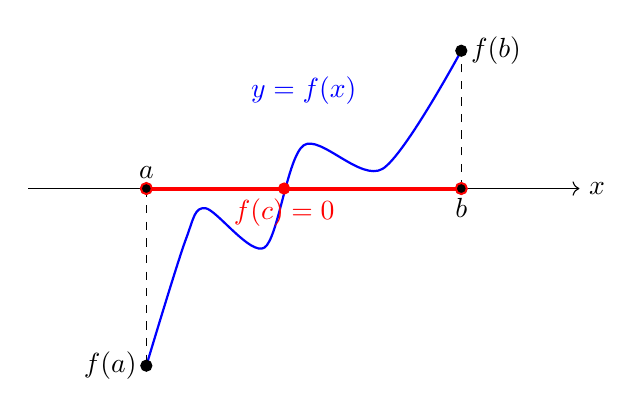
\begin{tikzpicture}[scale=1,domain=0:6]
	% Draw the axes
	\draw[->] (-0.5,-1.75) -- (6.5,-1.75) node[right] {$x$};
%	\draw[->] (0,-4) -- (0,0) node[above] {$f(x)$};
	
	% Define points a and b on the x-axis
	\coordinate (A) at (1,-1.75);
	\coordinate (B) at (5,-1.75);
	
	% Define points f(a), f(b) and gamma
	\coordinate (FA) at (1,-4); % f(a)
	\coordinate (FB) at (5,0); % f(b)
	\coordinate (GAMMA) at (0,2.5); % gamma horizontal line
	
	% Function graph
	\draw[color=blue,thick,smooth] plot coordinates {(1,-4) (1.5,-2.4) (1.75,-2) (2.5,-2.5) (3,-1.2) (4,-1.5) (5,0)};
	\node[blue] at (3,-.5) {$y=f(x)$};
	
	% Points on the graph
	\filldraw[black] (FA) circle (2pt) node[left] {$f(a)$};
	\filldraw[black] (FB) circle (2pt) node[right] {$f(b)$};
	
	% Draw vertical dashed lines for a and b
	\draw[dashed] (A) -- (FA);
	\draw[dashed] (B) -- (FB);
	
	% Labels for a and b
	\node[above] at (A) {$a$};
	\node[below] at (B) {$b$};
	
	\draw[red, line width=.5mm] (A) -- (B);
	\filldraw[black] (1,-1.75) circle (2pt);
	\filldraw[black] (5,-1.75) circle (2pt);
	
4	\draw[red, line width = .25mm] (1,-1.75) circle (2pt);
	\draw[red, line width = .25mm] (5,-1.75) circle (2pt);
	
	% Intersection point at c
	\filldraw[red] (2.75,-1.75) circle (2pt) node[below] {$f(c) = 0$};
\end{tikzpicture}

	\end{center}
\end{observation}
\vfill
\thmbox[Intermediate Value Theorem]{\begin{theorem*}
	Let $[a,b]\subseteq\mathbb{R}$ be a real interval, and let $f:[a,b]\to\mathbb{R}$ be a continuous function on $[a,b]$. Let $f(a)<f(b)$. If $\gamma\in\mathbb{R}$ satisfies $f(a)<\gamma<f(b)$, then \[
	\exists c\in(a,b)\ \text{such that}\ f(c)=\gamma.
	\] \begin{center}
		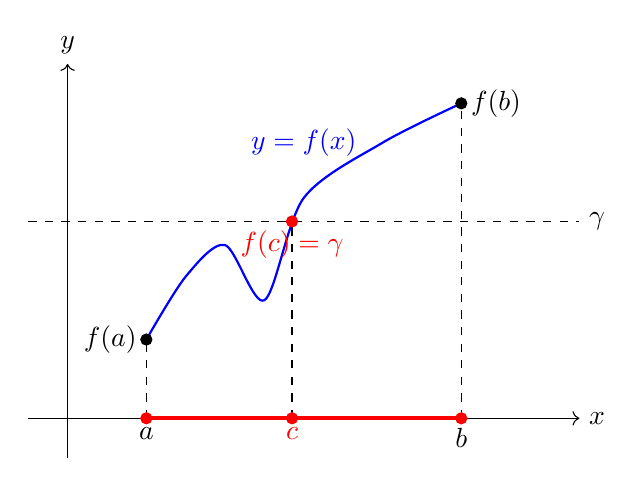
\begin{tikzpicture}[scale=1,domain=0:6,
	circledtail/.style={
		circle, draw, fill=white, inner sep=0pt, minimum size=6pt
	},
	open-open/.style={
		postaction={decorate, decoration={
				markings, 
				mark=at position 0 with {\node[circledtail]{};},  % Open circle at the start
				mark=at position 1 with {\node[circledtail]{};}   % Open circle at the end
		}}
	},
	closed-closed/.style={
		postaction={decorate, decoration={
				markings, 
				mark=at position 0 with {\filldraw[black] circle[radius=3pt];},  % Filled circle at start
				mark=at position 1 with {\filldraw[black] circle[radius=3pt];}   % Filled circle at end
		}}
	},
	open-closed/.style={
		postaction={decorate, decoration={
				markings, 
				mark=at position 0 with {\node[circledtail]{};},  % Open circle at the start
				mark=at position 1 with {\filldraw[black] circle[radius=3pt];}  % Filled circle at the end
		}},
		-{Stealth[scale=1.2]}
	},
	closed-open/.style={
		postaction={decorate, decoration={
				markings, 
				mark=at position 0 with {\filldraw[black] circle[radius=3pt];},  % Filled circle at the start
				mark=at position 1 with {\node[circledtail]{};}  % Open circle at the end
		}}
	}]
	% Draw the axes
	\draw[->] (-0.5,0) -- (6.5,0) node[right] {$x$};
	\draw[->] (0,-0.5) -- (0,4.5) node[above] {$y$};
	
	% Define points a and b on the x-axis
	\coordinate (A) at (1,0);
	\coordinate (B) at (5,0);
	
	% Define points f(a), f(b) and gamma
	\coordinate (FA) at (1,1); % f(a)
	\coordinate (FB) at (5,4); % f(b)
	\coordinate (GAMMA) at (0,2.5); % gamma horizontal line
	
	% Function graph
	\draw[color=blue,thick,smooth] plot coordinates {(1,1) (1.5,1.8) (2,2.2) (2.5,1.5) (3,2.8) (4,3.5) (5,4)};
	\node[blue] at (3,3.5) {$y=f(x)$};
		
	% Points on the graph
	\filldraw[black] (FA) circle (2pt) node[left] {$f(a)$};
	\filldraw[black] (FB) circle (2pt) node[right] {$f(b)$};
		
	% Draw vertical dashed lines for a and b
	\draw[dashed] (A) -- (FA);
	\draw[dashed] (B) -- (FB);
	
	% Labels for a and b
	\node[below] at (A) {$a$};
	\node[below] at (B) {$b$};
	
	\filldraw[red] (1,0) circle (2pt);
	\filldraw[red] (5,0) circle (2pt);
	\draw[red, line width=.5mm] (A) -- (B);
	
	% Gamma line and label
	\draw[dashed] (-0.5,2.5) -- (6.5,2.5) node[right] {$\gamma$};
	
	% Intersection point at c
	\draw[dashed] (2.85,0) -- (2.85,2.5);
	\filldraw[red] (2.85,2.5) circle (2pt) node[below] {$f(c) = \gamma$};
	\filldraw[red] (2.85,0) circle (2pt) node[below] {$c$};	
\end{tikzpicture}

	\end{center}
\end{theorem*}}
%\begin{remark*}
%\end{remark*}

\newpage
\tableofcontents
\vfill
\section{Numbers}
\begin{center}
\begin{tabular}{ll}
	$\N=\set{1,2,3,4,\dots}$ & \textbf{N}atural Numbers \\ \\
	$\Z=\set{0,\pm1,\pm2,\pm3,\pm4,\dots}$ & Integers (\textbf{Z}ahlen\footnotemark[1]) \\ \\
	$\Q=\set{\frac{q}{p}:p,q\in\Z,p\neq 0}$ & Rationals (\textbf{Q}uotient\footnotemark[2]) \\ \\
	$\R=\set{\text{Limit of sequences of rational numbers}}$ & \mathcolorbox{-red}{\text{\textbf{R}eal Numbers}} \\ \\
	$\C=\set{p+q\sqrt{-1}:p,q\in\R}$ & \textbf{C}omplex numbers
\end{tabular}
\addtocounter{footnote}{2}
\footnotetext[1]{The integer set is denoted by $\Z$ because it comes from the German word ``Zahlen'', meaning ``numbers''.}
\footnotetext[2]{The rational set is denoted by $\Q$ because it stands for ``Quotient'', representing numbers that can be expressed as the quotient of two integers.}
\end{center}
\vfill
\begin{remark*}
	The set $\mathbb{Z}_{\geq 0}:=\set{0}\cup\N=\set{0,1,2,\dots}$ is called \textit{non-negative integers}.
\end{remark*}
\begin{remark*}
	Let $n_0\in\Z$ is given. Then \[
	\Z_{\geq n_0}:=\set{n\in\Z:n\geq n_0}.
	\]
\end{remark*}

\section{Least Upper Bound Property of $\mathbb{R}$}
\defbox[Boundedness]{\begin{definition*}
	Let $S$ be a non-empty subset of $\R$.
	\begin{enumerate}[(1)]
		\item A set $S$ is said to be \hl{\textbf{bounded above}} if $
		\boxed{\exists \beta\in\mathbb{R}\ \text{such that for all}\ x\in S,\ x\leq \beta}$.\\ A real number $\beta\in\R$ is called an \hl{\textbf{upper bound}} of $S$.
		\item A set $S$ is said to be \hl{\textbf{bounded below}} if $\boxed{\exists \alpha\in\mathbb{R}\ \text{such that for all}\ x\in S,\ \alpha\leq x}$.\\ A real number $\alpha\in\R$ is called an \hl{\textbf{lower bound}} of $S$.
		\item A set $S$ is \hl{\textbf{bounded}} if it is bounded above and below.
	\end{enumerate}
\end{definition*}}
\begin{center}
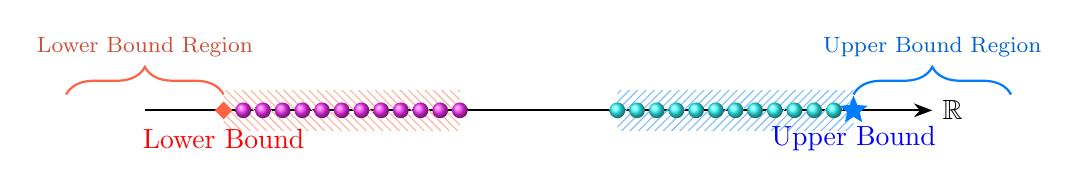
\begin{tikzpicture}[>=Stealth]
	\definecolor{upperboundcolor}{RGB}{0, 123, 255}   % Light blue for upper bound
	\definecolor{lowerboundcolor}{RGB}{255, 99, 71}   % Light coral for lower bound
	\definecolor{setcolor}{RGB}{34, 139, 34}          % Forest green for elements in set S
	
	% Draw the number line
	\draw[->, thick] (0, 0) -- (10, 0) node[right] {$\R$};
	
	% Diagonal patterned regions for lower and upper bounds
	\fill[pattern=north west lines, pattern color=lowerboundcolor!50] (1, -.25) rectangle (4, 0.25);
	\fill[pattern=north east lines, pattern color=upperboundcolor!50] (6, -.25) rectangle (9, 0.25);
	
	% Label and mark lower bound with a unique shape
	\node[draw=lowerboundcolor, fill=lowerboundcolor, diamond, inner sep=1.5pt, label=below:{\textcolor{red}{Lower Bound}}] at (1, 0) {};
	
	% Label and mark upper bound with a unique shape
	\node[draw=upperboundcolor, fill=upperboundcolor, star, star points=5, star point ratio=2.25, inner sep=1.5pt, label=below:{\textcolor{blue}{Upper Bound}}] at (9, 0) {};
	
	% Draw gradient elements within set S
	\foreach \x in {1.25, 1.5, ..., 4} {
		\shade[ball color=magenta!80!white] (\x, 0) circle (0.1);
	}
	\foreach \x in {6, 6.25, ..., 8.75} {
		\shade[ball color=cyan!80!white] (\x, 0) circle (0.1);
	}
	
	% Labels for the significance of bounds
%	\node[align=center, color=lowerboundcolor] at (2, 0.8) {No element \\ to the left};
%	\node[align=center, color=upperboundcolor] at (7, 0.8) {No element \\ to the right};
	
	% Curly braces to highlight bounds and elements of S
	\draw[decorate, decoration={brace, amplitude=10pt}, thick, color=lowerboundcolor] 
	(-1, 0.2) -- (1, 0.2) node[midway, above=10pt, color=lowerboundcolor!80!black] {\footnotesize Lower Bound Region};
%	\draw[decorate, decoration={brace, amplitude=10pt}, thick, color=gray] (2, 0.1) -- (5, 0.1)
%	node[midway, above=10pt, color=gray!80!black] {\( \varepsilon \)};
	
	\draw[decorate, decoration={brace, amplitude=10pt}, thick, color=upperboundcolor] 
	(9, 0.2) -- (11, 0.2) node[midway, above=10pt, color=upperboundcolor!80!black] {\footnotesize Upper Bound Region};
\end{tikzpicture}
\end{center}

\begin{remark*}[\textcolor{red}{\bf Caution!}]
	It is \textcolor{red}{not} guaranteed that $\beta\in S$ and $\alpha\in S$.
\end{remark*}
\vfill
\begin{remark*}
	Let $\varnothing\neq S\subseteq\R$, and let $\alpha,\beta\in\R$.
	\begin{align*}
		S\ \text{is bounded above}\ (\text{by}\ \beta) &\iff S\ \text{has an upper bound}\ \beta\\
		\beta\ \text{is an upper bound of}\ S &\iff \forall x\in S,\ x\leq \beta
	\end{align*}
	\begin{align*}
		S\ \text{is bounded below}\ (\text{by}\ \alpha) &\iff S\ \text{has an lower bound}\ \alpha\\
		\alpha\ \text{is an lower bound of}\ S &\iff \forall x\in S,\ \alpha\leq x
	\end{align*}
\end{remark*}
\vfill
\begin{remark*}
\ \begin{enumerate}
	\item The empty $S=\varnothing$ is bounded.
	\begin{enumerate}[(i)]
		\item ($\varnothing$ is bounded above) We need to find a real number $\beta\in\R$ s.t. for all $x\in\varnothing,\ x\leq\beta$. Since ``$\forall x\in\varnothing, x\leq\beta$'' is vacuously true, we can choose any real number as $\beta$.
		\item ($\varnothing$ is bounded below) Similarly, we can choose any $\alpha\in\R$ s.t. for all $x\in\varnothing$, $\alpha\leq x$.
	\end{enumerate}
	\item An upper bound and a lower bound may \underline{not be unique}. A set \( S(\neq\varnothing)\subseteq\R \) may have multiple upper bounds and multiple lower bounds.
\end{enumerate}
\end{remark*}
\newpage
\begin{exercise*}
Show that $A=\set{1-\frac{1}{n}:n\in\N}$ has an upper bound and a lower bound.
\begin{proof}[\sol]
	The elements of $A$ are: $A=\set{0, \frac{1}{2}, \frac{2}{3}, \frac{3}{4}, \frac{4}{5}, \cdots}$. Let $x\in A$. Then $x=1-1/n$ for some $n\in\N$. \begin{enumerate}[(i)]
		\item Since $n\in\mathbb{N}$, we have $1/n>0$. Therefore \[
		1-\frac{1}{n}<1.
		\] Thus, for all $x=1-1/n\in A$, we have $x\leq 1$. Hence $1$ be an upper bound of $A$.
		\item Since $n\in\N$, we have $n\geq 1$, so $1/n\leq 1$. Therefore, \[
		1-\frac{1}{n}\geq 1-1=0.
		\] Thus, for all $x=1-1/n\in A$, we have $x\geq 0$. Hence $0$ is a lower bound of $A$.
	\end{enumerate}
	\begin{center}
	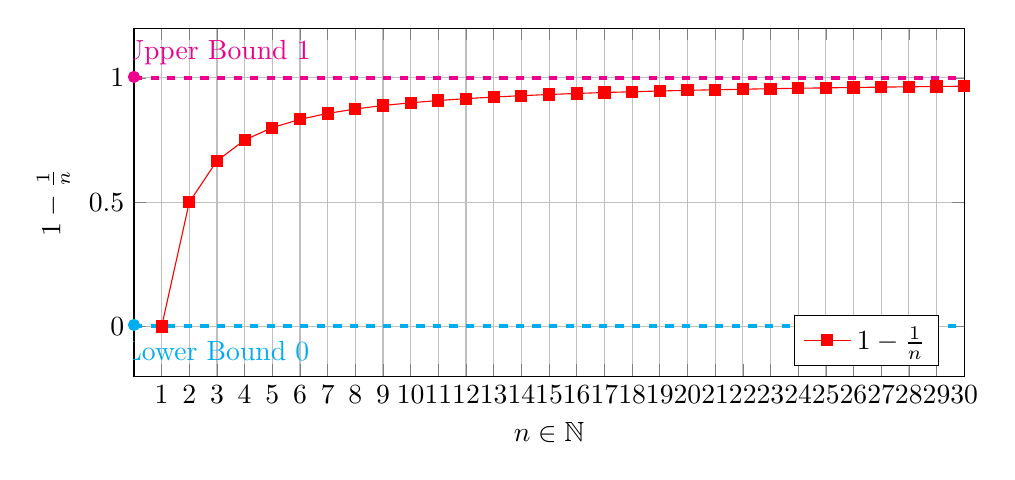
\begin{tikzpicture}
	\begin{axis}[
		xlabel={$n \in \mathbb{N}$},
		ylabel={$1 - \frac{1}{n}$},
		ymin=-.2, ymax=1.2,
		xmin=0, xmax=30,
		xtick={1,2,...,30},
		ytick={0,0.5,1},
		grid=major,
		width=\textwidth,
		height=6cm,
		domain=1:30,
		samples=30,
		legend pos=south east
		]
		% Plot points for 1 - 1/n
%		\addplot[line width=.25mm, only marks, red, mark=x] plot (\x, 1 - 1/\x);
		\addplot[red, mark=cube*, mark options={fill=red}] plot (\x, 1 - 1/\x);
		\addlegendentry{$1 - \frac{1}{n}$};
		
		% Draw horizontal line showing upper bound (y=1)
		\addplot[dashed, magenta, line width=.5mm] coordinates {(0,1) (30,1)};
		\node[magenta] at (axis cs: 3,1.1) {Upper Bound $1$};
		
		% Draw horizontal line showing lower bound (y=0)
		\addplot[dashed, cyan, line width=.5mm] coordinates {(0,0) (30,0)};
		\node[cyan] at (axis cs: 3,-0.1) {Lower Bound $0$};	
	\end{axis}
	\filldraw[magenta] (0,3.8) circle (2pt);
	\filldraw[cyan] (0,.65) circle (2pt);
\end{tikzpicture}
	\end{center}
\end{proof}
\end{exercise*}
\vfill
\begin{exercise*}
	Show that $\N$ has a lower bound but does not have an upper bound.
	\begin{proof}[\sol]
		Let $\N$ is the set of natural numbers. \begin{enumerate}[(i)]
			\item For each $n\in\N$, we have $n\geq 1$. Therefore, $1$ is a lower bound of $\N$.
			\item Assume that $\N$ is bounded above by $\beta\in\R$, \ie, \[
			\exists \beta\in\R\ \text{such that}\ \forall n\in\N,\ n\leq\beta.
			\]  However, for any $\beta\in\R$, we can always find $n\in\N$ s.t. $\beta < n$, by choosing $n=\floor{\beta} + 1 > \beta.$\\ It contradicts to the our assumption. Thus $\N$ does not have an upper bound.
		\end{enumerate}
	\end{proof}
\end{exercise*}
\begin{exercise*}[\textcolor{violet}{$\star$}]
	Consider a set \[
	A:=\set{r\in\Q:r>0,\ r^2<2}
	\] of positive rational numbers whose squares are less than 2. Then $A$ has a lower bound $0$. Prove that $A$ does not have the maximum element.
	\begin{proof}[\sol]
		Note that \[
		A:=\set{r\in\Q:r>0,\ r^2<2}=\set{\cdots,1.4, 1.41, 1.414, 1.4142, 1.41421, 1.4141213, 1.4142135, \cdots}.
		\] Let $a\in A$. Then \[
		a^2<2<4\implies a^2<4\implies\abs{a}<2\implies a < 2.
		\] That is, $A$ is bounded above by $2$. Suppose that $p$ is a maximum of $A$. Since $p\in A$, $p>0$ and $p^2<2$. 
		\begin{center}
		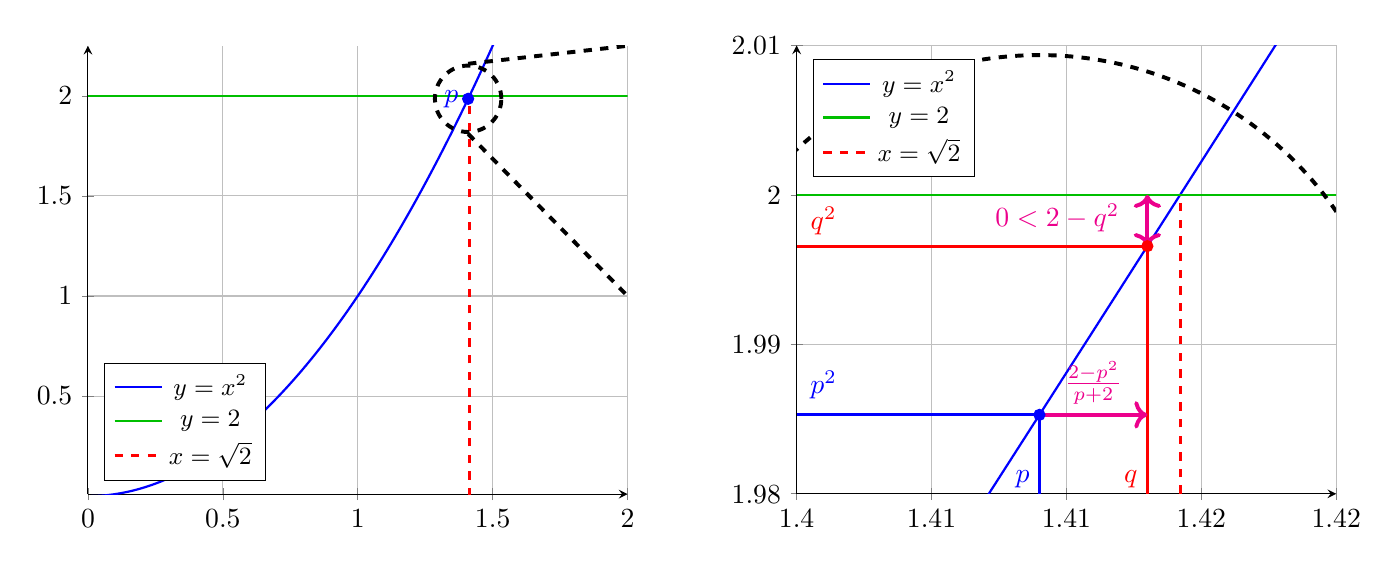
\begin{tikzpicture}[scale=1]
	\begin{scope}[xshift=-9cm]
	\begin{axis}[
		axis lines = left,
		xmin = 0, xmax = 2,
		ymin = 0.01, ymax = 2.25,
		domain=0:2,
		samples=1000,
		grid = both,
		legend pos=south west,
		legend style={font=\small},
		]
		
		% Plot m^2 curve
		\addplot[blue, thick] {x^2};
		\addlegendentry{$y=x^2$}
		
		% Plot line y=2
		\addplot[green!75!black, thick] {2};
		\addlegendentry{$y = 2$}
		
		\addplot[dashed, red, line width=.4mm] coordinates {(1.4142135, 0) (1.4142135, 2)};
		\addlegendentry{$x = \sqrt{2}$}
		
		% Mark an example point m
		\addplot[only marks, mark=*, blue] coordinates {(1.409,1.409^2)};
		\draw[dashed, line width=.5mm] (axis cs:1.409,1.409^2) circle (12pt);
		\draw[dashed, line width=.5mm] (axis cs:1.409,1.409^2-.175) -- (2,1);
		\draw[dashed, line width=.5mm] (axis cs:1.409,1.409^2+.175) -- (2,2.25);
		
%		\addplot[blue, line width=.4mm] coordinates {(1.409,0) (1.409, 1.409^2)} ;
		\node[anchor=east] at (axis cs:1.409,1.409^2) {$\textcolor{blue}{p}$};
%		\addplot[blue, line width=.4mm] coordinates {(1.4,1.409^2) (1.409, 1.409^2)};
%		\node[anchor=north] at (axis cs:1.401,1.9889) {$\textcolor{blue}{p^2}$};
	\end{axis}
	\end{scope}
	\begin{axis}[
		axis lines = left,
		xmin = 1.40, xmax = 1.42,
		ymin = 1.98, ymax = 2.01,
		domain=1.40:1.42,
		samples=1000,
		grid = both,
		legend pos=north west,
		legend style={font=\small},
		]
		
		% Plot m^2 curve
		\addplot[blue, thick] {x^2};
		\addlegendentry{$y=x^2$}
		
		% Plot line y=2
		\addplot[green!75!black, thick] {2};
		\addlegendentry{$y = 2$}
		
		\addplot[dashed, red, line width=.4mm] coordinates {(1.4142135, 0) (1.4142135, 2)};
		\addlegendentry{$x = \sqrt{2}$}
		
		% Mark an example point m
		\addplot[only marks, mark=*, blue] coordinates {(1.409,1.409^2)};
		
		% Mark m' near m
		\addplot[only marks, mark=*, red] coordinates {(1.413,1.413^2)};
		\addplot[red, line width=.4mm] coordinates {(1.413,0) (1.413, 1.413^2)} ;
		\node[anchor=east] at (axis cs:1.413,1.981) {$\textcolor{red}{q}$};
		\addplot[red, line width=.4mm] coordinates {(1.4,1.413^2) (1.413, 1.413^2)};
		\node[anchor=north] at (axis cs:1.401,1.9999) {$\textcolor{red}{q^2}$};
		
		\addplot[<->, line width=.5mm, magenta] coordinates {(1.413,1.413^2) (1.413, 2)};
		\node[anchor=west] at (axis cs:1.407,1.9985) {$\textcolor{magenta}{0<2-q^2}$};
		
		\addplot[blue, line width=.4mm] coordinates {(1.409,0) (1.409, 1.409^2)} ;
		\node[anchor=east] at (axis cs:1.409,1.981) {$\textcolor{blue}{p}$};
		\addplot[blue, line width=.4mm] coordinates {(1.4,1.409^2) (1.409, 1.409^2)};
		\node[anchor=north] at (axis cs:1.401,1.9889) {$\textcolor{blue}{p^2}$};
		
		% Arrow showing the increment
		\draw[->, line width=.5mm, magenta] (axis cs:1.409,1.409^2) -- (axis cs:1.413,1.409^2)
		node[midway, above, sloped] {\(\frac{2-p^2}{p+2}\)};
		
		\draw[dashed, line width=.5mm] (axis cs:1.409,1.409^2) circle (130pt);
	\end{axis}
\end{tikzpicture}
		\end{center}
		Define a rational number $q\in\Q$, for contradiction, by \[
		q:=p + \frac{2-p^2}{p+2}=\frac{2p+2}{p+2},	
		\] where $p<q$. We must show that $q\in A$. 
		\newpage
		\noindent Clearly $q>0$. We claim that $q^2<2$: \begin{align*}
			2-q^2=2-\left(p + \frac{2-p^2}{p+2}\right)^2
			&=2-\left(p^2+\frac{2p(2-p^2)}{p+2}+\frac{(2-p^2)^2}{(p+2)^2}\right) \\
			&=2-p^2-\frac{2p(2-p^2)}{p+2}-\frac{(2-p^2)^2}{(p+2)^2} \\
			&=\frac{(2-p^2)(p+2)^2-2p(2-p^2)(p+2)-(2-p^2)^2}{(p+2)^2} \\
%			&=\frac{1}{(p+2)^2}\left[(2-p^2)(p^2+4p+4)-(2p^2+4p)(2-p^2)-(p^4-4p^2+4)\right] \\
			&=\frac{1}{(p+2)^2}\left[(2-p^2)(p^2+4p+4)+(2p^2+4p)(p^2-2)+(-p^4+4p^2-4)\right] \\
			&=\frac{1}{(p+2)^2}\left[\crossout[red]{0}{(-1+2-1)p^4}+\crossout[red]{0}{(-4+4)p^3}+(2-4-\ncrossout[red]{4}+\ncrossout[red]{4})p^2+\crossout[red]{0}{(8-8)p}+(8-4)\right] \\
			&=\frac{1}{(p+2)^2}\left[-2p^2+4\right] =\frac{2(2-p^2)}{(p+2)^2}>0.
			\end{align*}
		Thus, $q\in A$ with $p<q$. It contradicts to the assumption that $p=\max A$. Hence it is proved.
	\end{proof}
\end{exercise*}
%\vfill
\vfill
\begin{note}[Existence of $\sqrt{2}$]
	There exists $x\in\R$ such that $x^2=2$. We write $x=\sqrt{2}>0$.
	\begin{proof}
		\textcolor{gray!50}{Consider a set \[
		A=\set{x\in\Q:x>0,\ x^2<2}\subseteq\R.
		\] Since $1\in A$, we know $A\neq\varnothing$. Clearly, $A$ is bounded above (by 2). \underline{By the completeness axiom}, $A$ has the supremum $\lambda=\sup A\in\R$.
%		By trichotomy, \[
%		\lambda^2=2,\quad \lambda^2>2\quad \text{or}\quad \lambda^2<2.
%		\]
		Define a number $\mu\in\R$ by\[
		\mu:=\lambda+\frac{2-\lambda^2}{\lambda+2},\ \text{and then}\ \mu^2-2=\frac{2(\lambda^2-2)}{(\lambda+2)^2}.
		\] \begin{enumerate}[(\text{Case} I)]
			\item Let $\lambda^2<2$. Then $\lambda <\mu$ and $\mu^2<2$. That is, $\mu\in A$ with $\lambda <\mu$.
			It contradicts to the fact that $\lambda$ is an upper bound of A.
			\item Let $\lambda^2>2$. Then \begin{align*}
				\mu<\lambda\ \text{and}\ 2 < \mu^2 \implies \forall x\in A,\ x^2<2<\mu^2
				&\implies \forall x\in A,\ x<\mu\\
				&\implies \mu\ \text{is an upper bound of}\ A\ \text{with}\ \mu <\lambda.
			\end{align*} It contradicts to the fact that $\lambda$ is an upper bound of $A$.
		\end{enumerate} By trichotomy, we obtain $\lambda^2=2$ with $\lambda\in\R$.}
	\end{proof}
\end{note}
\newpage
\defbox[Supremum and Infimum]{\begin{definition*}
	Let $\varnothing\neq S\subseteq\R$.
	\begin{enumerate}[(1)]
		\item Let $S$ is bounded above. The number $\beta\in\R$ is the \hl{\textbf{supremum}} (or the \hl{\textbf{least upper bound}}) of $S$ if and only if \begin{enumerate}[(i)]
			\item $\beta$ is an upper bound of $S$, \ie, $\forall x\in S,\ x\leq\beta$;
			\item $u$ is any upper bound of $S\implies \beta\leq u$.
		\end{enumerate} We write $\mathcolorbox{-red}{\beta=\sup S}\in\R$.
		\item Let $S$ is bounded below. The number $\alpha\in\R$ is the \hl{\textbf{infimum}} (or the \hl{\textbf{greatest lower bound}}) of $S$ if and only if \begin{enumerate}[(i)]
			\item $\alpha$ is an lower bound of $S$, \ie, $\forall x\in S,\ \alpha\leq x$;
			\item if $\ell$ is any lower bound of $S$ then $\ell\leq\alpha$.
		\end{enumerate} We write $\mathcolorbox{-red}{\alpha=\inf S}\in\R$.
	\end{enumerate}
\end{definition*}}
\begin{remark*}[\textcolor{red}{\bf Caution!}]
	It is \textcolor{red}{not} guaranteed that $\sup S\in S$ and that $\inf S\in S$.
\end{remark*}
\begin{remark*}
	Let $\varnothing\neq S\subseteq\mathbb{R}$. \begin{enumerate}[(1)]
		\item Suppose $S$ is bounded above. Then \begin{align*}
			\beta=\sup S \iff&\text{(i)}\ \forall x\in S, x\leq\beta;\\
			&\text{(ii)}\ \forall\text{upper bound}\ u\in S,\ \beta\leq u.
		\end{align*}
		\item Suppose $S$ is bounded below. Then \begin{align*}
			\alpha=\inf S \iff&\text{(i)}\ \forall x\in S, \alpha\leq x;\\
			&\text{(ii)}\ \forall \text{lower bound}\ \ell\in S,\ \ell\leq \alpha.
		\end{align*}
	\end{enumerate} 
\end{remark*}
\begin{remark*}
	\begin{align*}
		[u\ \text{is any upper bound of}\ S\implies \beta\leq u]&\iff [u<\beta\implies u\ \text{is NOT an upper bound of}\ S]\\
		&\iff \beta\leq u\ \text{for all upper bound $u$ of $S$}.
	\end{align*}
	\begin{align*}
		[\ell\ \text{is any lower bound of}\ S\implies \ell\leq\alpha]&\iff [\alpha<\ell\implies\ell\ \text{is NOT an lower bound of}\ S]\\
		&\iff \ell\leq \alpha\ \text{for all lower bound $\ell$ of $S$}.
	\end{align*}
\end{remark*}
\newpage
\begin{remark*}[\bf Uniqueness of Supremum and Infimum]
	\ \vspace{12pt} \\
	(\textit{Proof by \hyperlink{trichotomy}{Trichotomy}}) Let $\varnothing\neq S\subseteq\mathbb{R}$ and $S$ is bounded above. Suppose that $\sup S=a$ and that $\sup S=b$ also. By trichotomy, exactly one of the following holds: \[
	a=b,\ a<b,\ \text{or}\ b<a.  
	\] However, $a<b$ and $b<a$ are impossible, as $a$ and $b$ are upper bounds, respectively. Hence $a=b$. Similarly, infimum also is unique.\qed\vspace{12pt} \\
	(\textit{Proof by Anti-symmetry}\footnotemark[3]\textit{ of $\leq$})
	\addtocounter{footnote}{1}
	\footnotetext[3]{A relation $\mathcal{R}$ on a set $S$ is anti-symmetric if, for $a,b\in\mathcal{R}$, $a\relation b\land b\relation a\implies a=b$.}
	Let $\varnothing\neq T\subseteq\mathbb{R}$ and $T$ is bounded above. Suppose that $\sup T=a$ and that $\sup T=b$ also. Then \begin{center}\setstretch{1.5}
		\begin{tabular*}{\textwidth}{ll}
			(a) $a$ is an upper bound of $T$ in $\R$;
			& (b) $a$ is a supremum of $T$ in $\R$; \\
			(c) $b$ is an upper bound of $T$ in $\R$;
			& (d) $b$ is a supremum of $T$ in $\R$.
		\end{tabular*}
	\end{center} Then \[
	\text{(a) and (d)} \implies b\leq a,\quad\quad\quad\text{(b) and (c)} \implies a\leq b.
	\] By the anti-symmetry of $\leq$, we obtain $a=b$. Similarly, infimum also is unique.\qed
\end{remark*}
\vfill
\defbox[Unbounded Sets]{\begin{definition*}
Let $\varnothing\neq S\subseteq\R$. \begin{enumerate}[(1)]
	\item If $S$ is unbounded above, then we write $\boxed{\sup S=\infty}$.
	\item If $S$ is unbounded below, then we write $\boxed{\inf S=-\infty}$.
	\item $\sup\varnothing:=-\infty$ and $\inf\varnothing:=\infty$.
\end{enumerate}
\end{definition*}}
\begin{example*}
	$\sup \N=\infty$ and $\inf\Z=-\infty$.
\end{example*}
\begin{remark*}
	Suppose that $\varnothing\neq S\subseteq\R$ is unbounded above. Then \[
	\lnot[\exists\beta\in\R\ \text{s.t.}\ \forall x\in S,\ x\leq\beta],\quad \ie,\quad [\forall\beta\in\R,\ \exists x\in S\ \text{s.t.}\ \beta <x].
	\] Suppose that $\varnothing\neq T\subseteq\R$ is unbounded below. Then \[
	\lnot[\exists\alpha\in\R\ \text{s.t.}\ \forall x\in T,\ \alpha\leq x],\quad \ie,\quad [\forall\alpha\in\R,\ \exists x\in T\ \text{s.t.}\ x < \alpha].
	\]
\end{remark*}

\newpage
\probox[Approximation Property for Supremum and Infinum I]{\begin{proposition}
\ \hypertarget{pro1}{\begin{enumerate}[(1)]
	\item Let $\varnothing\neq S\subseteq\R$ which is bounded above, and let $\lambda$ be an upper bound of $S$ in $\R$. \[
	\lambda=\sup S\iff \forall\varepsilon>0,\ \exists x_\varepsilon\in S\ \text{s.t.}\ \lambda-\varepsilon<x_\varepsilon\leq\lambda.
	\]
	\item Let $\varnothing\neq T\subseteq\R$ which is bounded below, and let $\gamma$ be a lower bound of $T$ in $\R$. \[
	\gamma=\inf T\iff\forall\varepsilon>0,\ \exists x_\varepsilon\in T\ \text{s.t.}\ \gamma\leq x_\varepsilon<\gamma+\varepsilon.
	\]
\end{enumerate}}
\end{proposition}}
\begin{proof}
	\begin{enumerate}[(1)]
		\item \begin{itemize}
			\item[($\Rightarrow$)] Let $\lambda=\sup S$. Let $\varepsilon>0$. Suppose that \[
			\lnot[\exists x_\varepsilon\in S\ \text{s.t.}\ \lambda-\varepsilon<x_\varepsilon],\quad\ie,\quad[\forall x_\varepsilon\in S,\ x_\varepsilon\leq\lambda-\varepsilon].
			\] Then $\lambda-\varepsilon$ be an upper bound of $S$. Since $\varepsilon>0$, we have $\lambda-\varepsilon<\lambda$. It contradicts to the assumption that $\lambda$ is the \textit{least} upper bound of $S$. Thus \[
			\exists x_\varepsilon\in S\ \text{s.t.}\ \lambda-\varepsilon< x_\varepsilon.
			\] Since $x_\varepsilon\in S$ and $\lambda$ is an upper bound of $S$,  $x_\varepsilon\leq\lambda$ holds.
			\vspace{20pt}
			\item[($\Leftarrow$)] Let the RHS holds. We claim that $\lambda$ is the \textit{least} upper bound of $S$:\par
				\begin{center}
				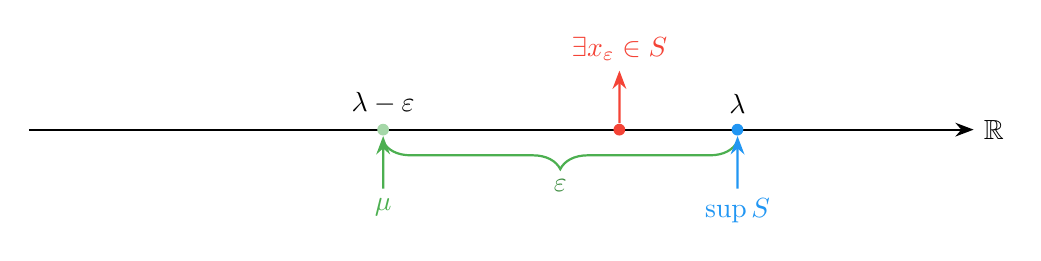
\begin{tikzpicture}[>=Stealth, scale=1.5]
	\definecolor{supcolor}{RGB}{33, 150, 243}       % Blue for supremum
	\definecolor{epsiloncolor}{RGB}{76, 175, 80}    % Green for epsilon interval
	\definecolor{pointcolor}{RGB}{244, 67, 54}      % Red for point in S
	
	% Draw the number line
	\draw[->, thick] (0, 0) -- (8, 0) node[right] {$\R$};
	
	% Mark the supremum point lambda
	\node[fill=supcolor, circle, inner sep=1.5pt, label=above:{\(\lambda\)}] (sup) at (6, 0) {};
	
	% Draw the interval (lambda - epsilon, lambda) with arrow to mark epsilon distance
	\node[fill=epsiloncolor!50, circle, inner sep=1.5pt, label=above:{\(\lambda - \varepsilon\)}] (epsilon) at (3, 0) {};
	\draw[decorate, decoration={brace, amplitude=10pt}, thick, color=epsiloncolor] (6, -0.1) -- (3, -0.1)
	node[midway, below=10pt, color=epsiloncolor!80!black] {\( \varepsilon \)};
	
	% Draw a point within the interval and label as x_epsilon
	\node[fill=pointcolor, circle, inner sep=1.5pt] (point) at (5, 0) {};
	
	% Arrow pointing to the existence of a point x_epsilon
	\draw[->, color=pointcolor, thick] (point) -- ++(0, 0.5) node[anchor=south] {\( \exists x_\varepsilon \in S \)};
	
	\draw[<-, color=supcolor, thick] (sup) -- ++(0, -0.5) node[anchor=north] {\(\sup S\)};
	\draw[<-, color=epsiloncolor, thick] (epsilon) -- ++(0, -0.5) node[anchor=north] {\(\mu\)};
\end{tikzpicture}

				\end{center}
				Assume, for contradiction, that there exists a smaller upper bound $\mu\in\R$ s.t. $\mu<\lambda$.\par
				Let $\varepsilon=\lambda-\mu>0$. Then \[
				\exists x_\varepsilon\in S\ \text{such that}\ \lambda-\varepsilon <x_\epsilon\leq\lambda,
				\] and so \[
				\mu=\lambda-\varepsilon <x_\varepsilon\leq\lambda\implies \mu <x_\varepsilon\leq\lambda.
				\] It contradicts to the assumption that $\mu$ is an upper bound of $S$. Thus, $\lambda$ be the least upper bound of $S$.
		\end{itemize}
		\newpage
		\item \begin{itemize}
			\item[($\Rightarrow$)] Let $\gamma=\inf T$. Let $\varepsilon>0$. Suppose that \[
			\lnot[\exists x\in T\ \text{s.t.}\ x<\gamma+\varepsilon],\quad\ie,\quad[\forall x\in T,\ \gamma+\varepsilon\leq x].
			\] Then $\gamma+\varepsilon$ be a lower bound of $T$. Since $\varepsilon>0$,  we have $\gamma<\gamma+\varepsilon$. It contradicts to the assumption that $\gamma$ is the \textit{greatest} lower bound of $T$. Thus, \[
			\exists x_\varepsilon\in T\ \text{s.t.}\ x_\varepsilon<\gamma+\varepsilon.
			\]
			Since $x_\varepsilon\in T$ and $\gamma$ is a lower bound of $T$, $\gamma\leq x_\varepsilon$ holds.
			\vspace{10pt}
			\item[($\Leftarrow$)] Let the RHS holds. We claim that $\gamma$ is the \textit{greatest} lower bound of $T$:\par
				\begin{center}
					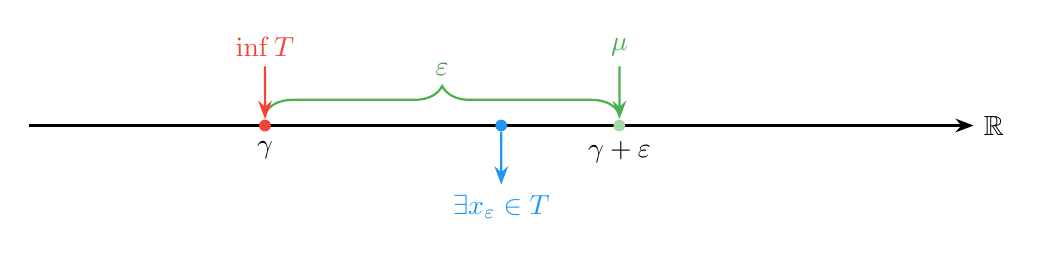
\begin{tikzpicture}[>=Stealth, scale=1.5]
	% Define colors for clarity
	\definecolor{infcolor}{RGB}{244, 67, 54}       % Red for infimum
	\definecolor{epsiloncolor}{RGB}{76, 175, 80}   % Green for epsilon interval
	\definecolor{pointcolor}{RGB}{33, 150, 243}    % Blue for point in T
	
	% Draw the number line
	\draw[->, thick] (0, 0) -- (8, 0) node[right] {$\R$};
	
	% Mark the infimum point gamma
	\node[fill=infcolor, circle, inner sep=1.5pt, label=below:{\(\gamma\)}] (inf) at (2, 0) {};
	
	% Draw the interval (gamma, gamma + epsilon) with arrow to mark epsilon distance
	\node[fill=epsiloncolor!50, circle, inner sep=1.5pt, label=below:{\(\gamma + \varepsilon\)}] (epsilon) at (5, 0) {};
	\draw[decorate, decoration={brace, amplitude=10pt}, thick, color=epsiloncolor] (2, 0.1) -- (5, 0.1)
	node[midway, above=10pt, color=epsiloncolor!80!black] {\( \varepsilon \)};
		
	% Draw a point within the interval and label as x_epsilon
	\node[fill=pointcolor, circle, inner sep=1.5pt] (point) at (4, 0) {};
	
	% Arrow pointing to the existence of a point x_epsilon
	\draw[->, color=pointcolor, thick] (point) -- ++(0, -0.5) node[anchor=north] {\( \exists x_\varepsilon\in T \)};
	
	\draw[<-, color=infcolor, thick] (inf) -- ++(0, 0.5) node[anchor=south] {\(\inf T\)};
	\draw[<-, color=epsiloncolor, thick] (epsilon) -- ++(0, 0.5) node[anchor=south] {\(\mu\)};
\end{tikzpicture}
				\end{center}
				Assume, for contradiction, that there exists a greater lower bound $\gamma<\mu$.\par
				Let $\varepsilon=\mu-\gamma>0$. Then \[
				\exists x_\varepsilon\in T\ \text{such that}\ \gamma\leq x_\varepsilon<\gamma+\varepsilon,
				\] and so $ \gamma \leq x_\varepsilon<\mu$. It contradicts to the assumption that $\gamma$ is an lower bound of $T$. Thus, $\gamma$ be the greatest lower bound of $T$.
		\end{itemize}
	\end{enumerate}
\end{proof}

\begin{remark*}
	See \hyperlink{pro2}{\bf Approximation Property for Supremum and Infinum II}.
\end{remark*}
\vfill
\axiombox[Least Upper Bound Property (Completeness Axiom) of Real Number]{\begin{axiom*}
	Every non-empty subset of $\R$ that is bounded above has the \underline{supremum} in $\R$.
\end{axiom*}}
\begin{example*}
	$\Q$ does NOT hold completeness axiom. We already showed that $\set{x\in\Q:x>0,\ x^2<2}$ has NO supremum in $\Q$.
\end{example*}
\vfill
\axiombox[Infimum Property]{\begin{axiom*}
	Every non-empty subset of $\R$ that is bounded below has the \underline{infimum} in $\R$.
\end{axiom*}}

\newpage
\section{Well-Ordering Principle and Mathematical Induction}
\axiombox[Well-Ordering Principle (Principle of the Least Element)]{\begin{axiom*}
	\hypertarget{wop}{Every non-empty subset $S$ of $\N$ has a least element, \ie, \[
	\varnothing\neq S\subseteq\N\implies\exists n\in S\ \text{s.t.}\ \forall k\in S,\ n\leq k.
	\] In other words, $[\varnothing\neq S\subseteq\N\Rightarrow\exists n\in S\ \text{s.t.}\ n=\min(S)$].}
\end{axiom*}}
\begin{remark*}[general version]
	\textcolor{gray!50}{$\varnothing\neq S\subseteq\Z_{\geq n_0}\implies\exists n\in S\ \text{s.t.}\ n=\min S\geq n_0$.}
\end{remark*}
%\begin{proof}
%	Since $\emptyset\neq S\subseteq\mathbb{N}$, we have $-S\subseteq\mathbb{Z}$. Then $-1$ be an upper bound of $-S$, that is, $-S$ is bounded above. By the completeness axiom of $\mathbb{R}$, $\exists\sup(-S)\in\mathbb{R}$. Moreover, $\sup(-S)\in -S$ because $-S\subseteq\mathbb{Z}$. By the reflection principal, $\exists -\sup(-S)=\inf(S)\in -(-S)=S$.
%\end{proof}
\vfill
\axiombox[Principle of Mathematical Induction]{\begin{axiom*}
	\hypertarget{mi}{Suppose that $S\subseteq\N$ satisfies the following two conditions: \begin{enumerate}
		\item (Basic Step) $1\in S$, and
		\item (Inductive Step) $n\in S\implies n+1\in S$.
	\end{enumerate} Then $S=\N$.}
\end{axiom*}}
\begin{remark*}[general version]
	\textcolor{gray!50}{Let $n_0\in\Z$ be given, and let $S\subseteq\Z_{\geq n_0}$. Suppose that $S$ satisfies the following two conditions: \begin{enumerate}
		\item (Basic Step) $n_0\in S$, and
		\item (Inductive Step) $\forall n\in\Z_{\geq n_0}: [n\in S\implies n+1\in S]$.
	\end{enumerate} Then $\forall n\in\Z_{\geq n_0}:n\in S$, \ie, $S=\Z_{\geq n_0}$.}
\end{remark*}
\vfill
\begin{remark*}
	To show that a mathematical statement $P(n)$ (property for $n$) holds for $n\in\N$, simply verify that the set \[
	S:=\set{n\in\N:P(n)\ \text{holds}}
	\] satisfies the following conditions: \begin{enumerate}[(\text{Step} 1)]
		\item Show that $P(1)$ holds.
		\item Show that $P(n+1)$ holds with the assumption $P(n)$ holds.
	\end{enumerate}
\end{remark*}
%\begin{example}
%	Show that \[
%	1+2+\cdots+n=\frac{n(n+1)}{2}
%	\] for all $n\in\ N$.
%	\begin{proof}[\sol]
%	\ \begin{enumerate}[(\text{Step} 1)]
%		\item (Basic Step) Let $n=1$. Then \[
%		\text{RHS}=1=\text{RHS}.
%		\]
%		\item (Inductive Step) Suppose that $1+2+\cdots k=\frac{k(k+1)}{2}$ for $n=k$. Then \[
%		1+2+\cdots+k+1=\frac{(k+1)(k+2)}{2}.
%		\]
%	\end{enumerate}
%	\end{proof}
%\end{example}

\newpage
\thmbox[Equivalence of Well-Ordering Principle and Induction]{\begin{theorem*}
	\ \begin{center}
	The \hyperlink{wop}{Well-Ordering Principle} and \hyperlink{mi}{Principle of Mathematical Induction} are equivalent.
	\end{center}
\end{theorem*}}
\begin{proof}
	\textbf{(WOP $\Rightarrow$ MI)}\ Let $S\subseteq\N$ satisfy the followings: (i) $1\in S$ and (ii) $k\in S\Rightarrow k+1\in S$. We want to establish that $S=\N$ by the Well-Ordering Principle (WOP). \par
	Assume for contradiction that $S\neq\N$. Then $S\subsetneq\N$, which means $\N\setminus S\neq\emptyset$. By the WOP, \[
	\exists m\in\N\setminus S\ \text{s.t.}\ m=\min(\N\setminus S).
	\] Since $1\in S$, we have $1\notin\N\setminus S$, so $m\neq 1$ and thus $m>1$ (or $m\geq 2$). 
	\begin{center}
	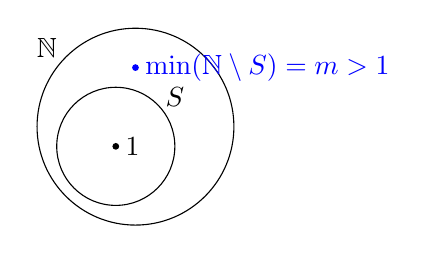
\begin{tikzpicture}[scale=.5]
	\draw (0,0) circle (2.5cm);
	\node at (-2.25,2) {$\N$};
	\draw (-.5,-.5) circle (1.5cm);
	\filldraw (-.5,-.5) circle (2pt) node[right] {$1$};
	\node at (1,.75) {$S$};
	\filldraw[blue] (0,1.5) circle (2pt) node[right] {$\min(\N\setminus S)=m>1$};
\end{tikzpicture}
	\end{center}
	Then \[
		m=\min(\N\setminus S)\overset{\textcolor{red}{\text{by minimality of}\ m}}{\implies} m-1\notin\N\setminus S \implies m-1\in S
		\overset{\text{by (ii)}}{\implies} m\in S\ \text{\Large\lightning}.
	\] Hence $S=\N$.\\
	\ \\
	\noindent \textbf{(MI $\Rightarrow$ WOP)}\ Suppose that $\varnothing\neq S\subseteq\N$ has no least element. Define the set $T\subseteq\N$ by \[
	T:=\set{n\in\N:1,2,3,\dots,n\notin S}.
	\]  For example, if $3\in T$ then $1,2,3\notin S$; conversely, if $1,2,3\notin S$ then $3\in T$. We claim that $T$ satisfies the condition of MI: \begin{enumerate}[(i)]
		\item (Basic Step) Since $S$ has no least element, $1\notin S$. Therefore, $1\in T$.
		\item (Inductive Step) Suppose that $k\in T$. This means that $1,2,\dots, k\notin S$. Since $S$ has no least element, $k+1\notin S$ (otherwise $k+1$ would be a least element of $S$). Therefore \[
		1,2,\dots,k,k+1\notin S,\ \ie,\ k+1\in T.
		\]
	\end{enumerate}
	By the Principle of Mathematical Induction, we have $T=\N$. It follows that no natural number is in $S$, which contradicts $S\neq\varnothing$. Hence it is proved.
\end{proof}

\section{Archimedean Principle}
\thmbox[Archimedean Property (The Unboundedness of Natural Numbers)]{\begin{theorem*}
	Let $x\in\R$. Then \[
	\exists n\in\N\ \text{such that}\ x < n.
	\]
\end{theorem*}}
\begin{center}
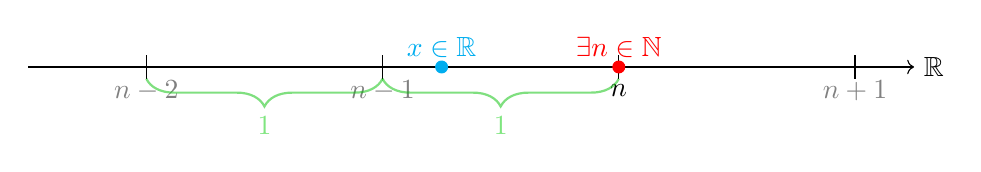
\begin{tikzpicture}[scale=1.5]
	% Draw the number line
	\draw[->] (-1, 0) -- (6.5, 0) node[right] {$\mathbb{R}$};
	
	% Mark points on the number line
	\foreach \x in {0, 2, ..., 6}
	\draw (\x,0.1) -- (\x,-0.1);
	
	% Mark point x
	\filldraw[cyan] (2.5, 0) circle (0.05) node[above] {$x\in\R$};
	
	% Mark point n
	\filldraw[red] (4, 0) circle (0.05) node[above] {$\exists n\in\N$};
	
	\node[gray] at (6,-0.2) {$n+1$};
	\node[] at (4,-0.2) {$n$};
	\node[gray] at (2,-0.2) {$n-1$};
	\node[gray] at (0,-0.2) {$n-2$};
	
	\draw[decorate, decoration={brace, amplitude=10pt}, thick, color=green!75!black, opacity=.5] (4, -0.1) -- (2, -0.1) 
	node[midway, below=10pt, color=green!80!black] {\( 1 \)};	
	\draw[decorate, decoration={brace, amplitude=10pt}, thick, color=green!75!black, opacity=.5] (2, -0.1) -- (0, -0.1) 
	node[midway, below=10pt, color=green!80!black] {\( 1 \)};	
\end{tikzpicture}
\end{center}
\begin{proof}
Assume, for contradiction, that \[
\forall n\in\N,\ n\leq x.
\] That is $\N\subseteq\R$ is bounded above by $x\in\R$. \underline{By the completeness axiom of $\R$}, \[
\exists\sup\mathbb{N}=:s\in\mathbb{R}.
\] By \hyperlink{pro1}{\textbf{Proposition 1}}, for $\varepsilon=1>0$, $\exists n\in\mathbb{N}$ s.t. $s-1<n$. Then \[
s-1<n\implies s<n+1\overset{n+1\in\N}{\implies}s<n+1\leq\sup\N=s\ \text{\Large\lightning}.
\]
\end{proof}
\vfill
\corbox{\begin{corollary*}
	Let $x,y\in\R$ with $x>0$. Then $\exists n\in\N\ \text{such that}\ y<n\cdot x$.
\end{corollary*}}
\begin{proof}
	Since $\R$ is a field, we know $\frac{y}{x}\in\R$. By the Archimedean property, \[
	\exists n\in\N\ \text{such that}\ \frac{y}{x}<n,\ \ie,\ y<n\cdot x.
	\]
\end{proof}
\begin{center}
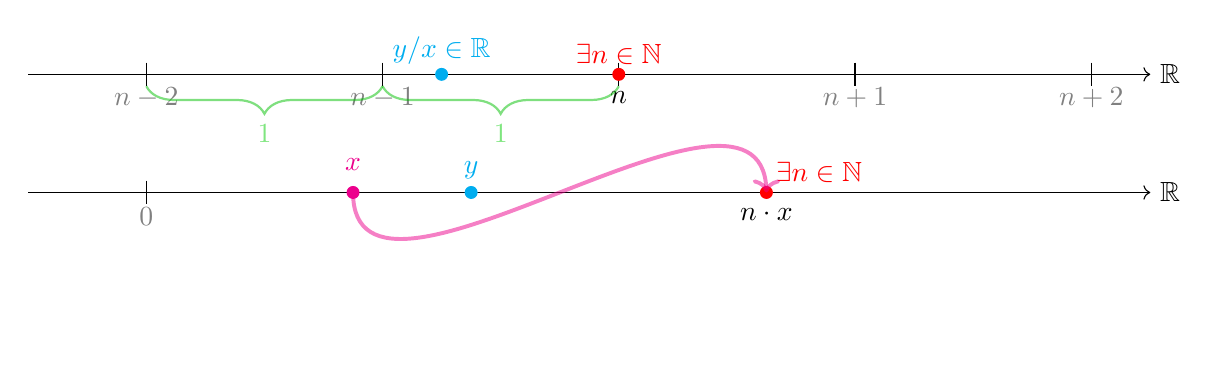
\begin{tikzpicture}[scale=1.5]
	\begin{scope}[yshift=1cm]
	\draw[->] (-1, 0) -- (8.5, 0) node[right] {$\mathbb{R}$};
	
	\foreach \x in {0, 2, ..., 8}
	\draw (\x,0.1) -- (\x,-0.1);
	
	\filldraw[cyan] (2.5, 0) circle (0.05) node[above] {$y/x\in\R$};
	\filldraw[red] (4, 0) circle (0.05) node[above] {$\exists n\in\N$};
	
	\node[gray] at (8,-0.2) {$n+2$};
	\node[gray] at (6,-0.2) {$n+1$};
	\node[] at (4,-0.2) {$n$};
	\node[gray] at (2,-0.2) {$n-1$};
	\node[gray] at (0,-0.2) {$n-2$};
	
	\draw[decorate, decoration={brace, amplitude=10pt}, thick, color=green!75!black, opacity=.5] (4, -0.1) -- (2, -0.1) 
	node[midway, below=10pt, color=green!80!black] {\( 1 \)};	
	\draw[decorate, decoration={brace, amplitude=10pt}, thick, color=green!75!black, opacity=.5] (2, -0.1) -- (0, -0.1) 
	node[midway, below=10pt, color=green!80!black] {\( 1 \)};
	\end{scope}
	% Draw the number line
	\draw[->] (-1, 0) -- (8.5, 0) node[right] {$\mathbb{R}$};
	
	% Mark points on the number line (multiples of x)
	\foreach \n in {0}
	\draw (\n, 0.1) -- (\n, -0.1);
	
	% Mark n * x point
	\filldraw[red] (5.25, 0) circle (0.05) node[above right] {$\exists n\in\N$};
	
%	\node[below, gray] at (8, -0.05) {$(n+1) \cdot x$};
	\node[below] at (5.25, -0.05) {$n \cdot x$};
%	\node[below, gray] at (4, -0.05) {$(n-1) \cdot x$};
%	\node[below, gray] at (2, -0.05) {$(n-2) \cdot x$};
	\node[below, gray] at (0, -0.05) {$0$};
	
	% Mark point y
	\filldraw[cyan] (2.75, 0) circle (0.05) node[above=.05cm] {$y$};
	\filldraw[magenta] (1.75, 0) circle (0.05) node[above=.15cm] {$x$};
	
	\draw[->, line width=.5mm, magenta,out=-90, in=90, opacity=.5] (1.75,0) to (5.25,0);
	
%	\draw[decorate, decoration={brace, amplitude=10pt}, thick, color=green!75!black, opacity=.5] (4, -0.1) -- (2, -0.1) 
%	node[midway, below=10pt, color=green!80!black] {\( x \)};	
%	\draw[decorate, decoration={brace, amplitude=10pt}, thick, color=green!75!black, opacity=.5] (2, -0.1) -- (0, -0.1) 
%	node[midway, below=10pt, color=green!80!black] {\( x \)};
\end{tikzpicture}
\end{center}
\corbox{\begin{corollary*}
$\forall\varepsilon>0,\ \exists n\in\N\ \text{such that}\ \frac{1}{n}<\varepsilon$.
\end{corollary*}}
\begin{proof}
	For $\varepsilon\in\R^+$ and $1\in\R$, by Archimedean property, we have \[
	\exists n\in\N\ \text{such that}\ 1<\varepsilon\cdot n,\ \ie, \frac{1}{n}<\varepsilon.
	\]
\end{proof}
\begin{center}
	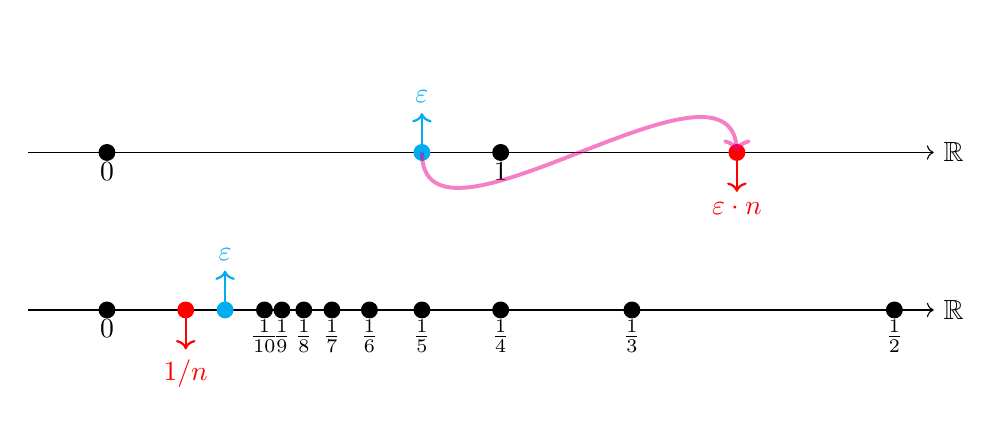
\begin{tikzpicture}[scale=2]
	\begin{scope}[yshift=1cm]
		\draw[->] (-0.5, 0) -- (5.25, 0) node[right] {$\mathbb{R}$};
		\filldraw[cyan] (2, 0) circle (0.05);
		\filldraw[red] (4, 0) circle (0.05);
		\filldraw[black] (2.5, 0) circle (0.05) node[anchor=north] {$1$};
		\filldraw[black] (0, 0) circle (0.05) node[anchor=north] {$0$};
		
		\draw[->, color=cyan, thick] (2,0) -- ++(0, +0.25) node[anchor=south] {\( \varepsilon \)};
		\draw[->, color=red, thick] (4,0) -- ++(0, -0.25) node[anchor=north] {\( \varepsilon\cdot n \)};
		
		\draw[->, color=magenta, line width=.5mm, in=90, out=-90, opacity=.5] (2,0) to (4,0);
	\end{scope}
	\draw[->] (-0.5, 0) -- (5.25, 0) node[right] {$\mathbb{R}$};
	\filldraw[cyan] (.75, 0) circle (0.05);
	\filldraw[red] (.5, 0) circle (0.05);
	\filldraw[black] (0, 0) circle (0.05) node[anchor=north] {$0$};
	
	% Set a value for epsilon on the number line
%	\pgfmathsetmacro{\eps}{0} % Position of epsilon
	
	% Define points for 1/n using calculations
	\foreach \n in {2, 3, ..., 10} {
		\pgfmathsetmacro{\pos}{10 / \n} % Scale positions for 1/n
		\draw[fill=black] (\pos, 0) circle (0.05) node[below] {$\frac{1}{\n}$};
	}

	\draw[->, color=cyan, thick] (.75,0) -- ++(0, +0.25) node[anchor=south] {\( \varepsilon \)};
	\draw[->, color=red, thick] (.5,0) -- ++(0, -0.25) node[anchor=north] {\( 1/n \)};	
		
%	\draw[decorate, decoration={brace, amplitude=10pt}, thick, color=green!75!black, opacity=.5] (5, -0.1) -- (10 / 3, -0.1) 
%	node[midway, below=10pt, color=green!80!black] {\( 1/6 \)};	
%	\draw[decorate, decoration={brace, amplitude=10pt}, thick, color=green!75!black, opacity=.5] (10/3, -0.1) -- (10/4, -0.1) 
%	node[midway, below=10pt, color=green!80!black] {\( 1/12 \)};
%	\draw[decorate, decoration={brace, amplitude=10pt}, thick, color=green!75!black, opacity=.5] (10/4, -0.1) -- (10/5, -0.1) 
%	node[midway, below=10pt, color=green!80!black] {\( 1/20 \)};	
\end{tikzpicture}

%\begin{tikzpicture}
%	% Draw the number line
%	\draw[->] (-0.5, 0) -- (8, 0) node[right] {$\mathbb{R}$};
%	
%	% Set a value for epsilon and scale positions for n * epsilon
%	\pgfmathsetmacro{\eps}{1} % Value of epsilon
%	
%	% Mark the value 1 on the number line
%%	\draw[fill=black] (1, 0) circle (0.05) node[above] {$1$};
%	
%	% Define points for n * epsilon using calculations
%	\foreach \n in {1, 2, 3, 4, 5, 6, 7} {
%		\pgfmathsetmacro{\pos}{\n * \eps} % Calculate position for n * epsilon
%		\draw[fill=black] (\pos, 0) circle (0.05) node[below] {$\n \cdot \varepsilon$};
%	}
%	
%	% Draw inequality arrow from 1 to the appropriate n*epsilon where 1 < n * epsilon
%%	\pgfmathsetmacro{\npos}{3 * \eps} % Position where 1 < n * epsilon (e.g., 3 * epsilon)
%%	\draw[thick, ->] (1.1, 0.3) -- (\npos - 0.1, 0.3) node[midway, above] {$1 < n \cdot \varepsilon$};
%	
%\end{tikzpicture}
\end{center}
%\begin{remark*}
%Let $x=\varepsilon>0$ and $y=1$. By Archimedean Property, \[
%\exists n\in\N\ \text{such that}\ 1<\varepsilon\cdot n\ \left(\Leftrightarrow \frac{1}{n}<\varepsilon\right).
%\]
%\end{remark*}
\vfill
\begin{note}[Archimedean Property in Number Theory]
	Let $a,b\in\mathbb{N}$. Then $
	\exists n\in\mathbb{N}\ \text{such that}\ b< na$.
%	\begin{tikzpicture}
%		% Draw the number line
%		\draw[->] (-1, 0) -- (10, 0) node[right] {$\mathbb{R}$};
%		
%		% Label points along the number line at multiples of a
%		\foreach \n in {1, 2, 3, 4, 5, 6, 7, 8}
%		\draw (\n, 0.1) -- (\n, -0.1) node[below] {\small $\n a$};
%		
%		% Mark the point b
%		\draw[fill=black] (3.5, 0) circle (0.05) node[above] {$b$};
%		
%		% Mark a point for n*a where b < n * a
%		\draw[fill=black] (6, 0) circle (0.05) node[above] {$n \cdot a$};
%		
%		% Draw inequality arrow for b < n * a
%		\draw[thick, ->] (3.6, 0.3) -- (5.9, 0.3) node[midway, above] {$b < n \cdot a$};
%		
%	\end{tikzpicture}
	\begin{proof}
	\textcolor{gray!50}{Suppose that $
	\exists a,b\in\mathbb{N}$ such that \[
	\forall n\in\N, na\leq b.
	\] Define a set $S$ by \[
	S:=\set{b-na\geq 0:n\in\mathbb{N}}\subseteq\Z_{\geq 0}.
	\] \underline{By the well-ordering principle}, $\exists s:=\min S$. Since $s=\min S\in S$, we have\[
	s=b-ma\ \text{for some}\ m\in\mathbb{N}.
	\] Since $m+1\in\N$ also, we have  $b-(m+1)a\in S$, and so \begin{align*}
		{b-(m+1)a}&=b-ma-a\\
		& {<}\ b-ma\quad\because a\in\N, \ie, a > 0\\
		& ={\min S}\ \text{\Large\lightning}.
	\end{align*} Hence it is proved. }
	\end{proof}	
\end{note}

\newpage
\probox[Approximation Property for Supremum and Infinum II]{\begin{proposition}
\ \hypertarget{pro2}{\begin{enumerate}[(1)]
		\item Let $\varnothing\neq S\subseteq\R$ which is bounded above, and let $\lambda$ be an upper bound of $S$ in $\R$. \begin{align*}
			\lambda=\sup S &\iff \forall\varepsilon>0,\ \exists x_\varepsilon\in S\ \text{s.t.}\ \lambda-\varepsilon<x_\varepsilon\leq\lambda \\
			&\iff \forall n\in\N,\ \exists x_n\in S\ \text{s.t.}\ \lambda-\frac{1}{n}<x_n\leq\lambda.
		\end{align*}
		\item Let $\varnothing\neq T\subseteq\R$ which is bounded below, and let $\gamma$ be a lower bound of $T$ in $\R$. \begin{align*}
		\gamma=\inf T\in\R &\iff\forall\varepsilon>0,\ \exists x_\varepsilon\in T\ \text{s.t.}\ \gamma\leq x_\varepsilon<\gamma+\varepsilon \\
		&\iff\forall n\in\N,\ \exists x_n\in T\ \text{s.t.}\ \gamma\leq x_n<\gamma+\frac{1}{n}.
		\end{align*}
\end{enumerate}}
\end{proposition}}
\begin{proof}
\begin{enumerate}[(1)]
	\item We NTS that \[
	[\forall\varepsilon>0,\ \exists x_\varepsilon\in S\ \text{s.t.}\ \lambda-\varepsilon<x_\varepsilon\leq\lambda]
	\iff [\forall n\in\N,\ \exists x_n\in S\ \text{s.t.}\ \lambda-\frac{1}{n}<x_n\leq\lambda].
	\] \begin{itemize}
		\item[($\Rightarrow$)] Assume that the LHS holds. Let $n\in\N$. Since $1/n>0$, we can take $\varepsilon=1/n$ for each $n\in\N$. By assumption, for this choice of $\varepsilon$, \[
		\exists x_n\in S\ \text{s.t.}\ \lambda-\frac{1}{n}< x_n\leq\lambda.
		\]
		\item[($\Leftarrow$)] Assume that the RHS holds. 
		\begin{center}
		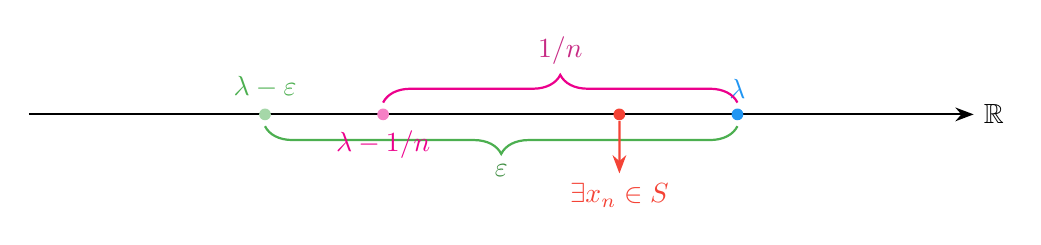
\begin{tikzpicture}[>=Stealth, scale=1.5]
	\definecolor{supcolor}{RGB}{33, 150, 243}       % Blue for supremum
	\definecolor{epsiloncolor}{RGB}{76, 175, 80}    % Green for epsilon interval
	\definecolor{pointcolor}{RGB}{244, 67, 54}      % Red for point in S
	
	% Draw the number line
	\draw[->, thick] (0, 0) -- (8, 0) node[right] {$\R$};
	
	% Mark the supremum point lambda
	\node[fill=supcolor, circle, inner sep=1.5pt, label=above:{\textcolor{supcolor}{\(\lambda\)}}] (sup) at (6, 0) {};
	
	% Draw the interval (lambda - epsilon, lambda) with arrow to mark epsilon distance
	\node[fill=epsiloncolor!50, circle, inner sep=1.5pt, label=above:{\textcolor{epsiloncolor}{\(\lambda - \varepsilon\)}}] (epsilon) at (2, 0) {};
	\draw[decorate, decoration={brace, amplitude=10pt}, thick, color=epsiloncolor] (6, -0.1) -- (2, -0.1)
	node[midway, below=10pt, color=epsiloncolor!80!black] {\( \varepsilon \)};
	
	\node[fill=magenta!50, circle, inner sep=1.5pt, label=below:{\textcolor{magenta}{\(\lambda - 1/n\)}}] (ap) at (3, 0) {};
	\draw[decorate, decoration={brace, amplitude=10pt}, thick, color=magenta] (3, 0.1) -- (6, 0.1)
	node[midway, above=10pt, color=magenta!80!black] {\( 1/n \)};	
	
	% Draw a point within the interval and label as x_epsilon
	\node[fill=pointcolor, circle, inner sep=1.5pt] (point) at (5, 0) {};
	
%	 Arrow pointing to the existence of a point x_epsilon
	\draw[->, color=pointcolor, thick] (point) -- ++(0, -0.5) node[anchor=north] {\( \exists x_n \in S \)};
	
%	\draw[<-, color=supcolor, thick] (sup) -- ++(0, -0.5) node[anchor=north] {\(\sup S\)};
%	\draw[<-, color=epsiloncolor, thick] (epsilon) -- ++(0, -0.5) node[anchor=north] {\(\mu\)};
\end{tikzpicture}
		\end{center}
		Let $\varepsilon>0$. By Archimedean property, $\exists n\in\N\ \text{s.t.}\ \frac{1}{n}<\varepsilon.$ By assumption, for this $n$, \[
		\lambda-\frac{1}{n}< x_n\leq\lambda.
		\] Since $1/n<\varepsilon$, we have $\lambda-\varepsilon<\lambda-\frac{1}{n},$ and so \[
			\lambda-\varepsilon<\lambda-\frac{1}{n}<x_n\leq\lambda,\ \text{\ie},\ \lambda-\varepsilon< x_n\leq\lambda.
		\] Letting $x_n=x_\varepsilon$, we see that such an $x_\varepsilon\in S$ exists for any $\varepsilon>0$.
	\end{itemize}
	\item We NTS that \[
	[\forall\varepsilon>0,\ \exists x_\varepsilon\in T\ \text{s.t.}\ \gamma\leq x_\varepsilon<\gamma+\varepsilon]
	\iff[\forall n\in\N,\ \exists x_n\in T\ \text{s.t.}\ \gamma\leq x_n<\gamma+\frac{1}{n}].
	\] \begin{itemize}
		\item[($\Rightarrow$)] Assume that the LHS holds. Let $n\in\N$. Since $1/n>0$, we can take $\varepsilon=1/n$ for each $n\in\N$. By assumption, for this choice of $\varepsilon$, \[
		\exists x_n\in T\ \text{s.t.}\ \gamma\leq x_n< \gamma+\varepsilon.
		\]
		\item[($\Leftarrow$)] Assume that the RHS holds. 
		\begin{center}
		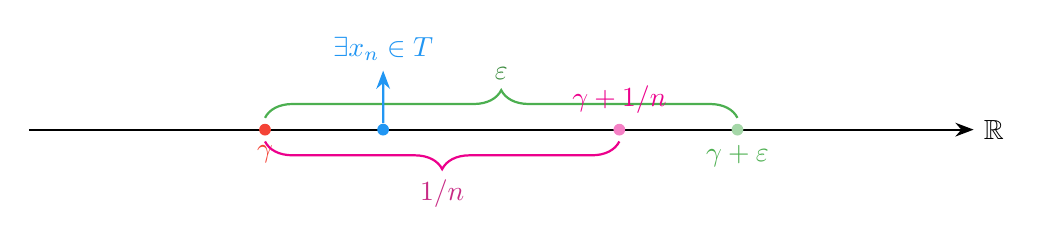
\begin{tikzpicture}[>=Stealth, scale=1.5]
	% Define colors for clarity
	\definecolor{infcolor}{RGB}{244, 67, 54}       % Red for infimum
	\definecolor{epsiloncolor}{RGB}{76, 175, 80}   % Green for epsilon interval
	\definecolor{pointcolor}{RGB}{33, 150, 243}    % Blue for point in T
	
	% Draw the number line
	\draw[->, thick] (0, 0) -- (8, 0) node[right] {$\R$};
	
	% Mark the infimum point gamma
	\node[fill=infcolor, circle, inner sep=1.5pt, label=below:{\textcolor{infcolor}{\(\gamma\)}}] (inf) at (2, 0) {};
	
	% Draw the interval (gamma, gamma + epsilon) with arrow to mark epsilon distance
	\node[fill=epsiloncolor!50, circle, inner sep=1.5pt, label=below:{\textcolor{epsiloncolor}{\(\gamma + \varepsilon\)}}] (epsilon) at (6, 0) {};
	\draw[decorate, decoration={brace, amplitude=10pt}, thick, color=epsiloncolor] (2, 0.1) -- (6, 0.1)
	node[midway, above=10pt, color=epsiloncolor!80!black] {\( \varepsilon \)};
	
	\node[fill=magenta!50, circle, inner sep=1.5pt, label=above:{\textcolor{magenta}{\(\gamma + 1/n\)}}] (epsilon) at (5, 0) {};
	\draw[decorate, decoration={brace, amplitude=10pt}, thick, color=magenta] (5, -0.1) -- (2, -0.1)
	node[midway, below=10pt, color=magenta!80!black] {\( 1/n \)};
	
	
	% Draw a point within the interval and label as x_epsilon
	\node[fill=pointcolor, circle, inner sep=1.5pt] (point) at (3, 0) {};
	
	% Arrow pointing to the existence of a point x_epsilon
	\draw[->, color=pointcolor, thick] (point) -- ++(0, 0.5) node[anchor=south] {\( \exists x_n\in T \)};
	
%	\draw[<-, color=infcolor, thick] (inf) -- ++(0, 0.5) node[anchor=south] {\(\inf T\)};
%	\draw[<-, color=epsiloncolor, thick] (epsilon) -- ++(0, 0.5) node[anchor=south] {\(\mu\)};
\end{tikzpicture}
		\end{center}
		Let $\varepsilon>0$. By Archimedean property, $\exists n\in\N\ \text{s.t.}\ \frac{1}{n}<\varepsilon$. By assumption, for this $n$, \[
		\gamma\leq x_n<\gamma+\frac{1}{n}.
		\] Since $1/n<\varepsilon$, we have $\gamma+\frac{1}{n}<\gamma+\varepsilon$, and so \[
		\gamma\leq x_n<\gamma+\frac{1}{n}<\gamma+\varepsilon,\ \text{\ie},\ \gamma\leq x_n<\gamma+\varepsilon.
		\] Letting $x_n=x_\varepsilon$, we see that such an $x_\varepsilon\in T$ exists for any $\varepsilon>0$.
	\end{itemize}
\end{enumerate}
\end{proof}
\begin{remark*}
	See \hyperlink{pro1}{\bf Approximation Property for Supremum and Infinum I}.
\end{remark*}
\vfill
\thmbox[Density of the Rationals]{\begin{theorem*}
	Let $a,b\in\mathbb{R}$. \[
	a<b\implies \exists q\in\mathbb{Q}\ \text{such that}\ a<q<b.
	\]
\end{theorem*}}
\begin{proof}
Let $a,b\in\mathbb{R}$. Suppose that $a<b$. 
\begin{center}
	\adjustbox{scale=.75}{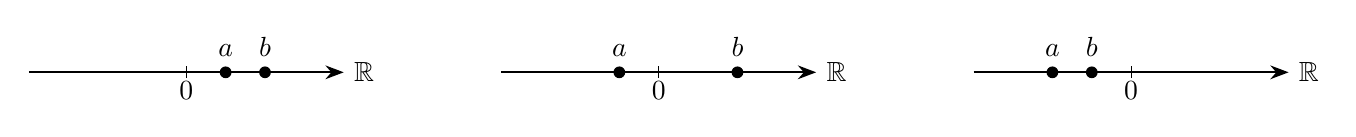
\begin{tikzpicture}[>=Stealth, scale=1]
	\draw[->, thick] (-2, 0) -- (2, 0) node[right] {$\R$};
	
	\node[fill=black, circle, inner sep=1.5pt, label=above:{$a$}] (a) at (0.5, 0) {};
	\node[fill=black, circle, inner sep=1.5pt, label=above:{$b$}] (b) at (1, 0) {};
	\draw (0,-.075) -- (0,.075) node[midway, below] {$0$};
	
	\begin{scope}[xshift=6cm]
	\draw[->, thick] (-2, 0) -- (2, 0) node[right] {$\R$};
	
	\node[fill=black, circle, inner sep=1.5pt, label=above:{$a$}] (a) at (-.5, 0) {};
	\node[fill=black, circle, inner sep=1.5pt, label=above:{$b$}] (b) at (1, 0) {};
	\draw (0,-.075) -- (0,.075) node[midway, below] {$0$};
	\end{scope}

	\begin{scope}[xshift=12cm]
		\draw[->, thick] (-2, 0) -- (2, 0) node[right] {$\R$};
		
		\node[fill=black, circle, inner sep=1.5pt, label=above:{$a$}] (a) at (-1, 0) {};
		\node[fill=black, circle, inner sep=1.5pt, label=above:{$b$}] (b) at (-.5, 0) {};
		\draw (0,-.075) -- (0,.075) node[midway, below] {$0$};
	\end{scope}
\end{tikzpicture}}
\end{center} We consider the following two cases: 
\begin{enumerate}[(\text{Case} I)]
	\item ($0\leq a$) Since $b-a>0$, we have $\frac{1}{b-a}\in\R$. By the \textcolor{red}{Archimedean property}, \[
	\exists \textcolor{red}{n}\in\mathbb{N}\quad \text{s.t.}\quad \frac{1}{b-a}<n,\ \text{\ie},\ na+1< nb.
	\] Clearly $na\in\R$. Define a set $A$ by \[
	A:=\set{k\in\N:na<k}\subseteq\mathbb{N}.
	\] By the Archimedean property, $\exists k\in\mathbb{N}$ such that $na<k$. That is, $A\neq\emptyset$. By the \textcolor{cyan}{well-ordering principle}, $\exists \textcolor{cyan}{m}=\min A$. By the minimality of $m$, we know $m-1\notin A$, \ie, $m-1\leq na$, and so $m\leq na+1$. Thus, we obtain \[
	na\overset{m\in A}{<}m\leq na+1\overset{\text{by A.P.}}{<}nb.
	\] Therefore \[
	na<m<ny\implies a<\frac{m}{n}<b.
	\] Thus, $q:=\frac{\textcolor{cyan}{m}}{\textcolor{red}{n}}\in\Q$ satisfies $a<q<b$.
	\item ($a<0$) Note that $-a\in\R^+$. By the Archimedean property, \[
	\exists n\in\mathbb{N}:-a<n,\ \text{\ie},\ 0<a+n.
	\] By (Case I), we have \[
	\exists q\in\mathbb{Q}: a+n<q<b+n
	\] since $0<a+n<b+n$. Let $q'=q-n\in\mathbb{Q}$. Then $a<q'<b$.
\end{enumerate}
\end{proof}
\vfill
\begin{thebibliography}{9}
	\bibitem{advanced_calc_a}
	수학의 즐거움, Enjoying Math. ``수학 공부, 기초부터 대학원 수학까지, 4. 해석학 개론 (a) 완비성 공리.'' YouTube Video, 32:20. Published 
	September 09, 2019. URL: \url{https://www.youtube.com/watch?v=pHIImTBdBRs}.
	\bibitem{advanced_calc_b}
	수학의 즐거움, Enjoying Math. ``수학 공부, 기초부터 대학원 수학까지, 5. 해석학 개론 (b) 유리수의 조밀성와 실수, 자연수 공리'' YouTube Video, 30:51. Published 
	September 11, 2019. URL: \url{https://www.youtube.com/watch?v=RYjhQyXxTpQ&t=2s}.
\end{thebibliography}

\newpage
\appendix
\section{Axioms of the Real Numbers}
%\begin{center}
%\begin{tikzpicture}
%	% Define positions of axioms and the real number
%	\node[draw, rectangle, minimum width=2cm, minimum height=1cm, fill=blue!10] (Field) at (0, 3) {Field Axiom};
%	\node[draw, rectangle, minimum width=2cm, minimum height=1cm, fill=green!10] (Order) at (-3, 1.5) {Order Axiom};
%	\node[draw, rectangle, minimum width=2cm, minimum height=1cm, fill=red!10] (Completeness) at (3, 1.5) {Completeness Axiom};
%	
%	% Draw the target "Real Number System" node
%	\node[draw, ellipse, minimum width=3cm, minimum height=1cm, fill=yellow!20] (RealNumber) at (0, 0) {\(\mathbb{R}\) (Real Numbers)};
%	
%	% Connect each axiom to the Real Number System
%	\draw[->, thick] (Field) -- (RealNumber);
%	\draw[->, thick] (Order) -- (RealNumber);
%	\draw[->, thick] (Completeness) -- (RealNumber);
%\end{tikzpicture}
%\end{center}
\begin{center}\resizebox{\textwidth}{!}{
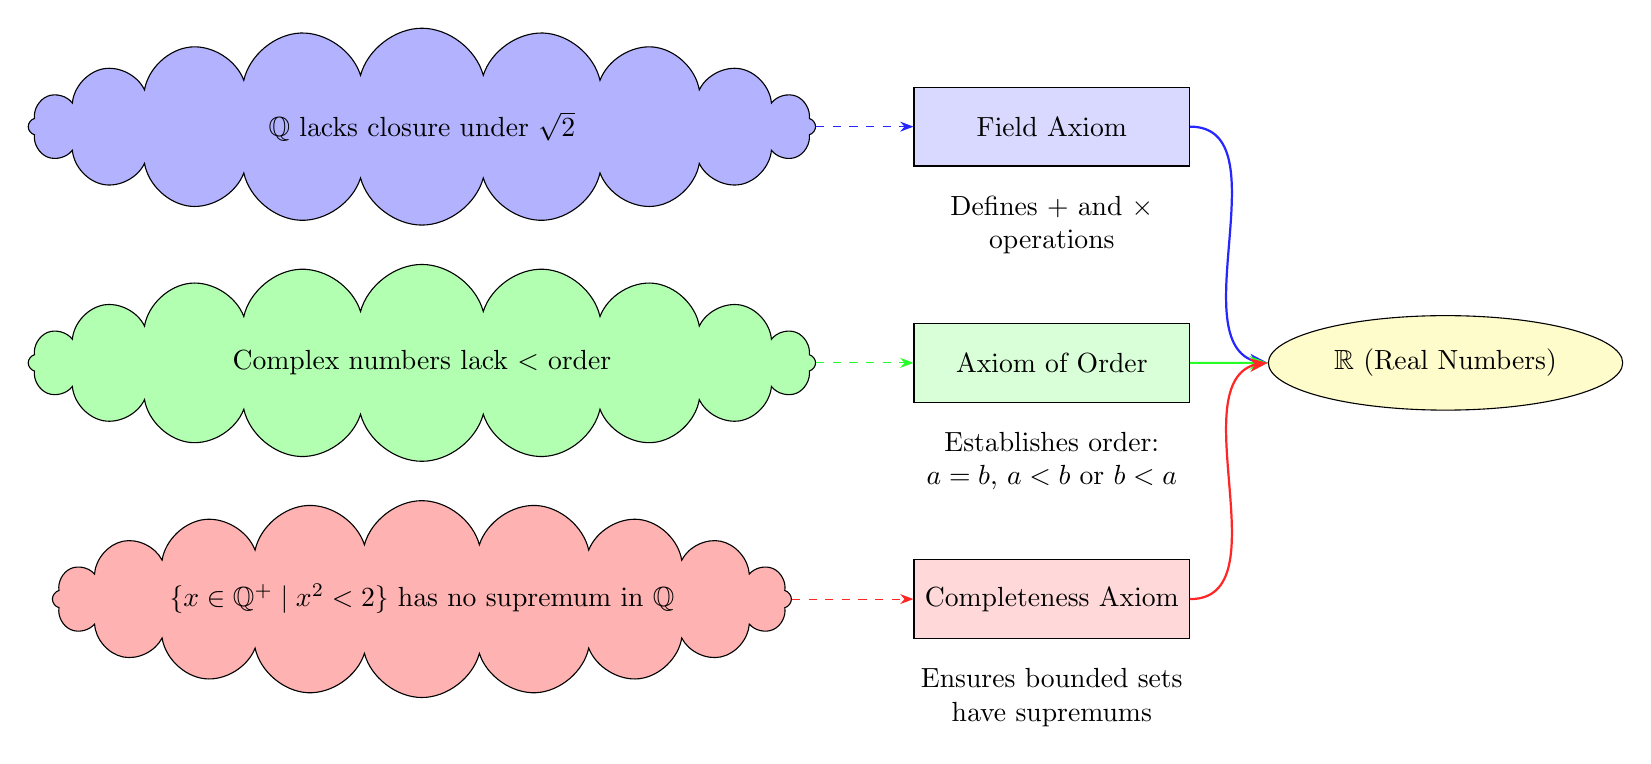
\begin{tikzpicture}[>=Stealth]
	% Define positions for axioms and examples of failure without them
	\node[draw, rectangle, minimum width=3.5cm, minimum height=1cm, fill=blue!15] (Field) at (1, 7) {Field Axiom};
	\node[draw, rectangle, minimum width=3.5cm, minimum height=1cm, fill=green!15] (Order) at (1, 4) {Axiom of Order};
	\node[draw, rectangle, minimum width=3.5cm, minimum height=1cm, fill=red!15] (Completeness) at (1, 1) {Completeness Axiom};
	
	% Define basic principles of each axiom
	\node[align=center] at (1, 5.75) {Defines $+$ and $\times$\\ operations};
	\node[align=center] at (1, 2.75) {Establishes order:\\$a=b$, $a < b$ or $b < a$};
	\node[align=center] at (1, -.25) {Ensures bounded sets\\have supremums};
	
	% Add visual examples of failures if each axiom is omitted
	\node[draw, cloud, cloud puffs=20, cloud ignores aspect, minimum width=10cm, minimum height=2.5cm, fill=blue!30, align=center] (FailField) at (-7, 7) {$\mathbb{Q}$ lacks closure under $\sqrt{2}$};
	\node[draw, cloud, cloud puffs=20, cloud ignores aspect, minimum width=10cm, minimum height=2.5cm, fill=green!30, align=center] (FailOrder) at (-7, 4) {Complex numbers lack $<$ order};
	\node[draw, cloud, cloud puffs=20, cloud ignores aspect, minimum width=4cm, minimum height=2.5cm, fill=red!30, align=center] (FailCompleteness) at (-7, 1) {$\{x \in \mathbb{Q}^+ \mid x^2 < 2\}$ has no supremum in $\Q$};
	
	% Draw the Real Numbers
	\node[draw, ellipse, minimum width=4.5cm, minimum height=1.2cm, fill=yellow!20] (RealNumber) at (6, 4) {\(\mathbb{R}\) (Real Numbers)};
	
	% Connect each axiom to Real Numbers and show necessity
	\draw[->, thick, in=180, out=0, blue!85] (Field) to (RealNumber);
	\draw[->, thick, in=180, out=0, green!85] (Order) to (RealNumber);
	\draw[->, thick, in=180, out=0, red!85] (Completeness) to (RealNumber);
	
	% Draw arrows from failure examples to each axiom
	\draw[->, dashed, blue!85] (FailField) -- (Field);
	\draw[->, dashed, green!85] (FailOrder) -- (Order);
	\draw[->, dashed, red!85] (FailCompleteness) -- (Completeness);
\end{tikzpicture}}
\end{center}
\noindent
The following axioms define the real numbers \(\mathbb{R}\) as a complete ordered field.

\subsection{Field Axioms}

\subsubsection*{Addition:}
\begin{enumerate}
	\item \textbf{Closure under addition}: $\forall a, b \in \mathbb{R}, \ a + b \in \mathbb{R}$
	\item \textbf{Associativity of addition}:$\forall a, b, c \in \mathbb{R}, \ (a + b) + c = a + (b + c)$
	\item \textbf{Commutativity of addition}:$\forall a, b \in \mathbb{R}, \ a + b = b + a$
	\item \textbf{Existence of additive identity}: $
	\exists 0 \in \mathbb{R} \ \text{such that} \ \forall a \in \mathbb{R}, \ a + 0 = a$
	\item \textbf{Existence of additive inverses}: $
	\forall a \in \mathbb{R}, \ \exists -a \in \mathbb{R} \ \text{such that} \ a + (-a) = 0$
\end{enumerate}
\subsubsection*{Multiplication:}
\begin{enumerate}
	\item \textbf{Closure under multiplication}: $\forall a, b \in \mathbb{R}, \ a \cdot b \in \mathbb{R}$
	\item \textbf{Associativity of multiplication}: $
	\forall a, b, c \in \mathbb{R}, \ (a \cdot b) \cdot c = a \cdot (b \cdot c)$
	\item \textbf{Commutativity of multiplication}: $
	\forall a, b \in \mathbb{R}, \ a \cdot b = b \cdot a$
	\item \textbf{Existence of multiplicative identity}: $
	\exists 1 \in \mathbb{R}, 1 \neq 0, \ \text{such that} \ \forall a \in \mathbb{R}, \ a \cdot 1 = a$
	\item \textbf{Existence of multiplicative inverses}: $
	\forall a \in \mathbb{R}, a \neq 0, \ \exists a^{-1} \in \mathbb{R} \ \text{such that} \ a \cdot a^{-1} = 1$
\end{enumerate}
\subsubsection*{Distributive law:}
\begin{enumerate}
	\item \textbf{Distributivity of multiplication over addition}: $
	\forall a, b, c \in \mathbb{R}, \ a \cdot (b + c) = a \cdot b + a \cdot c$
\end{enumerate}
\vspace{20pt}
\subsection{Axiom of Order}
A relation $<$ defined on $\R$ satisfy the followings:
\begin{enumerate}
	\item \hypertarget{trichotomy}{\textbf{Trichotomy}: 
	For $a,b\in\R$, \underline{exactly one} of the following holds: \[
	a=b,\quad a < b,\quad \text{or}\quad b < a.
	\]}
	\item \textbf{Transitivity}: For $a,b,c\in\R$,
	\[a < b \ \text{and} \ b < c \implies a < c\]
	\item \textbf{Additive compatibility}: For $a,b,c\in\R$,
	\[a < b \implies a + c < b + c\]
	\item \textbf{Multiplicative compatibility}: For $a,b\in\R$ and $c\in\R^+$,
	\[a < b \implies a \cdot c < b \cdot c\]
\end{enumerate}
\vspace{20pt}
\subsection{Completeness Axiom}
\textbf{The least upper bound property} (or \textbf{supremum property}): 
\[
\forall S\subseteq \mathbb{R}, \ S \neq \emptyset, \ \text{if} \ S \ \text{is bounded above}\ \text{then}\ \exists \sup(S) \in \mathbb{R}
\]

\newpage
\section{Application of Well-Ordering Principle}
\thmbox{\begin{theorem*}
	$\sqrt{2}$ is irrational, \ie, $\sqrt{2}\in\R\setminus\Q$.
\end{theorem*}}
\begin{proof}
	Suppose $\sqrt{2}\in\Q$. That is, $\exists p,q\in\N$ s.t. $p\sqrt{2}=q$. Define a set $S$ by \[
	S:=\set{k\sqrt{2}\in\N:k\in\N}\subseteq\N.
	\] Since $p\sqrt{2}=q\in\N$, we have $S\neq\varnothing$. By the Well-Ordering Principle, \[
	\exists s=\min (S)\in S.
	\] Then $s=t\sqrt{2}$ for some $t\in\N$. Define a number \[
	r:=s\sqrt{2}-s.
	\] \begin{enumerate}[(\text{Claim} 1)]
		\item $r\in S$: \begin{align*}
			r&=s\sqrt{2}-s\\
			&=s\sqrt{2}-t\sqrt{2}\\
			&=(s-t)\sqrt{2}\\
			&\in S &\because s=t\sqrt{2}>t\Rightarrow s-t>0\Rightarrow s-t\in\N.
		\end{align*}
		\item $r<s = \min(S)$: \begin{align*}
			r&=s\sqrt{2}-s\\
			&=s(\sqrt{2}-1)\\
			&<s=\min S &\because s\in\N\ \text{and}\ 1<\sqrt{2}<2\Rightarrow 0<\sqrt{2}-1<1.
		\end{align*}
	\end{enumerate}
	It is a contradiction. Hence $\sqrt{2}\notin\Q$.
\end{proof}
\newpage
\section{The 2nd Principle of Mathematical Induction}
\thmbox[The 2nd Principle of Mathematical Induction]{\begin{theorem*}\hypertarget{mi-2nd}{
Suppose that $T\subseteq\N$ satisfies the following two conditions: \begin{enumerate}
	\item (Basic Step) $1\in T$, and
	\item (Inductive Step) $1,2,\dots n\in T\implies n+1\in T$.
\end{enumerate} Then $T=\N$.}
\end{theorem*}}
\begin{proof}
	We use the first principle of mathematical induction. Define the set $T'$ by \[
	T':=\set{n\in\N:1,2,\dots,n\in T}\subseteq\N.
	\] For example, if $1,2,3\in T$ then $3\in T'$; conversely, if $3\in T'$ then $1,2,3\in T$. Since $n\in T'\Rightarrow n\in T$, we have $T'\subseteq T\subseteq\N$. We claim that $T'$ satisfies the condition of MI: \begin{enumerate}[(i)]
		\item (Basic Step) Clearly $1\in T'$.
		\item (Inductive Step) Suppose that $k\in T'$. This means that $1,2,\dots k\in T$. By condition 2, \[
		1,2,\dots,k,k+1\in T,\ \ie,\ k+1\in T'.
		\]
	\end{enumerate}  
	Therefore by the first principle of mathematical induction, $T'=\N$. That is, \[
	\N=T'\subseteq T\subseteq\N\implies T=\N.
	\] Hence it is proved.
\end{proof}
\vfill
\begin{remark*}
	To show that a mathematical statement \( P(n) \) (property for \( n \)) holds for \( n \in \mathbb{N} \), verify that the set
	\[
	S := \{ n \in \mathbb{N} : P(n) \text{ holds} \}
	\]
	satisfies the following conditions:
	\begin{enumerate}[(\text{Step} 1)]
		\item Show that \( P(1) \) holds.
		\item Show that \( P(n+1) \) holds assuming \( P(k) \) holds for all \( k \leq n \).
	\end{enumerate}
\end{remark*}
\end{document}
